\documentclass{article}

% if you need to pass options to natbib, use, e.g.:
%     \PassOptionsToPackage{numbers, compress}{natbib}
% before loading neurips_2020

% ready for submission
% \usepackage{neurips_2020}

% to compile a preprint version, e.g., for submission to arXiv, add add the
% [preprint] option:
%     \usepackage[preprint]{neurips_2020}

% to compile a camera-ready version, add the [final] option, e.g.:
%     \usepackage[final]{neurips_2020}

% to avoid loading the natbib package, add option nonatbib:
     \usepackage[]{neurips_2020}

\usepackage[utf8]{inputenc} % allow utf-8 input
\usepackage[T1]{fontenc}    % use 8-bit T1 fonts
\usepackage{hyperref}       % hyperlinks
\usepackage{url}            % simple URL typesetting
\usepackage{booktabs}       % professional-quality tables
\usepackage{amsfonts}       % blackboard math symbols
\usepackage{nicefrac}       % compact symbols for 1/2, etc.
\usepackage{microtype}      % microtypography
\usepackage{graphicx}
\usepackage{amsmath}

\usepackage{pythonhighlight}

\usepackage{algorithm}
\usepackage[noend]{algpseudocode}

\makeatletter
\def\BState{\State\hskip-\ALG@thistlm}
\makeatother

\title{Optimization for Total-Variation Image Denoising}

% The \author macro works with any number of authors. There are two commands
% used to separate the names and addresses of multiple authors: \And and \AND.
%
% Using \And between authors leaves it to LaTeX to determine where to break the
% lines. Using \AND forces a line break at that point. So, if LaTeX puts 3 of 4
% authors names on the first line, and the last on the second line, try using
% \AND instead of \And before the third author name.

\author{%
  Bingcheng HU \\
  Department of Electric and Computer Engneering\\
  Shanghai Jiao Tong University\\
  Student ID: 516021910219 \\
  \texttt{bingcheng@sjtu.edu.cn} \\
}

\begin{document}

\maketitle

\begin{abstract}
Nowadays, smartphones are generally equipped with high-definition cameras, and the effect of taking pictures at night is always unsatisfactory, because when the light is weak, the internal and external noises become relatively large. TV regularization is an algorithm that reduces data noise by processing data in different dimensions. In this paper, the optimization of the TV denoising algorithm for monochrome pictures is discussed.

Keywords: total variation, regularized learning, sparsity, convex optimization

\end{abstract}

\section{Introduction}

Total variation has a long history in the field of image processing, and it was originally a good solution for signal denoising problems [\citealp{Condat2013,Durand2003,Easley2008,Selesnick2014}]. \citet{Condat2013}  propose a fast denoising algorithm for filtering discrete signals using total variation regularization \citep{Condat2013}. The optimization problem of the one-dimensional (1D) discrete signals denoising is shown as below.
$$
\operatorname{min}_{x \in \mathbb{R}^{N}} \frac{1}{2} \sum_{k=1}^{N}|y[k]-x[k]|^{2}+\lambda \sum_{k=1}^{N-1}|x[k+1]-x[k]|
$$
where y is the noised signal and by solving this optimization problem, we can get the denoised signal x. \citet{Condat2013} presents an efficient way to implement this convex optimization problem, and one example of the usage of the algorithm in signal processing is shown in figure \ref {img1} \citep{Condat2013}.

\begin{figure}[h]
  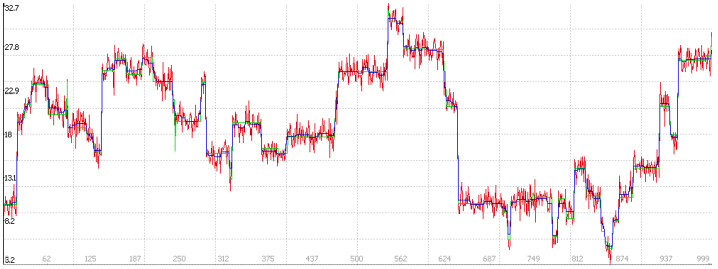
\includegraphics[width=5in]{pic1.png}
  \centering
  \caption{One example of the noised signal (in red) , the unknown ground truth (in green), and the TV-denoised signal x (in blue) \citep{Condat2013}.}
  \label{img1}
\end{figure}

Apart from the signal denoising, the total variance method was considered a well-established way to solve image processing problems [\citealp{Chen2010,Blomgren1997,Chen2015,Thanh2015}]. I real life, people need to take photos at night and their phones always catch a noised picture because of the lack of light. Nowadays, many smartphone companies introduced lots of algorithms to improve the quality of the photo (\citealp{Chen2010,Blomgren1997,Chen2015}). In those algorithms, the total variant is still a very important part of denoising.

In the photograph field, Total variant denoising can help the photographer get a better picture. But for non-professionals, it is difficult to adjust the regularization parameter. \citet{Chen2010} proposed a majorization-minimization approach for adaptative total variation image denoising. Using their methods, regularization parameter doesn't need to be specified by authors. This layman-friendly method can easily make total variant image denoising expand into daily life. Figure \ref {img2} shows the practical application of this algorithm. The picture shows a picture of a zebra. The picture on the left is the original picture, and the picture with noize added in the middle. On the right is the image after noise reduction using the total variant denoising. By carefully comparing Figure 1.c and Figure 1.a, you can find that the denoised image has an excellent performance in detail retention.

\begin{figure}[h]
  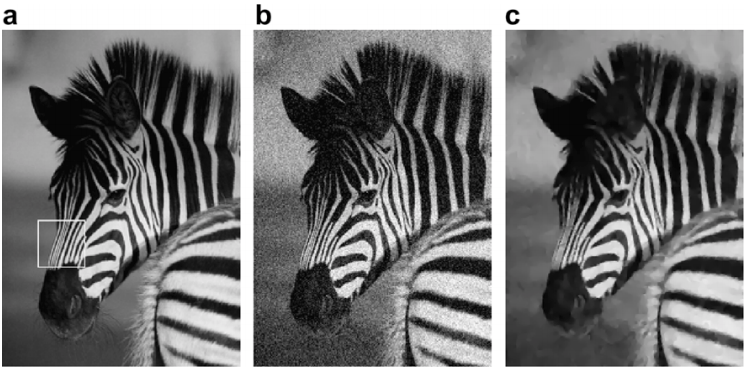
\includegraphics[width=5in]{pic2.png}
  \centering
  \caption{One example of the original image (a) , the noised image (b), and the TV-denoised image (c) \citep{Chen2010}.}
  \label{img2}
\end{figure}

Total variant image denoising is also a significant part of medical imaging. \citet{Thanh2015} proposes a TV denoising algorithm for biomedical images. This algorithm achieves noise reduction in line with medical standards by adjusting parameters. This noise reduction method will retain important details such as blood vessels, so that the details will not be erased by the noise reduction algorithm. However, this algorithm will cause color distortion, so it can not be used to denoise everyday photos. Figure \ref {img3} shows the MRI pictures of the human brain before and after noise reduction. Observing the pictures shows that the details of the images are well preserved.

\begin{figure}[h]
  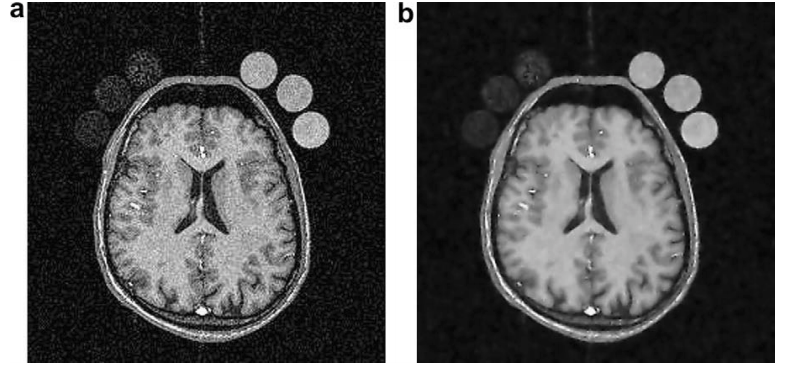
\includegraphics[width=3.5in]{pic3.png}
  \centering
  \caption{One example of the original noised image of the human brain scanned image (a) , and the TV-denoised image (b) \citep{Thanh2015}.}
  \label{img3}
\end{figure}

In the field of total variant denoising, lots of new technologies were introduced these years. Many of them can achieve high quality, while still some algorithms were too slow for use in daily life []. \citet{Blomgren1997} studies  one of the most useful images restoring algorithm and the optimization illustration of its problem is shown as below \citep{Blomgren1997}.
$$
\min _{u} \alpha T V(u)+\frac{1}{2}\|\mathbb{K} u-z\|_{\mathcal{L}^{2}}^{2}
$$
The Total Variation norm chosen in this equation is $TV(u) = \int_{\Omega}|\nabla u| d x d y$. Because the Total Variation norm does not penalize disruption in $u$ , it ensures a better restoration for edges\citep{Blomgren1997}.

\citet{Beck2009}  introduced gradient-based strategies for image denoising and deblurring problems, and the model of the algorithm is based on TV minimization model with constraints \citep{Beck2009}. The innovative invention of this paper is the usage of a fast iterative shrinkage/thresholding algorithm (FISTA) with its "novel monotone version” \citep{Beck2009}. The convex non-smooth minimization problem is represented as below.
$$
\min _{\mathbf{x}}|\mathcal{A}(\mathbf{x})-\mathbf{b}\|^{2}+2 \lambda \mathrm{T} \mathrm{V}(\mathbf{x}), \quad(\lambda>0)
$$
Where $TV(·)$ stands for the l1-based, anisotropic TV, which is defined by
$$
\begin{aligned}
\mathbf{x} \in \mathbb{R}^{m \times n}, \quad \mathrm{T} \mathrm{V}_{l_{1}}(\mathbf{x})=& \sum_{i=1}^{m-1} \sum_{j=1}^{n-1}\left\{\left|x_{i, j}-x_{i+1, j}\right|+\left|x_{i, j}-x_{i, j+1}\right|\right\} \\
&+\sum_{i=1}^{m-1}\left|x_{i, n}-x_{i+1, n}\right|+\sum_{j=1}^{n-1}\left|x_{m, j}-x_{m, j+1}\right|
\end{aligned}
$$
which is more complex than we have learned in class.

\citet{Chen2015} invented the fractional-order TV denoising model. The given image is denoted as the function $f: \Omega \rightarrow \mathbb{R}$, where $\Omega$ is the subset of $R^2$ in the image domain and the fractional-order TV denoising model is described by
$$
\min _{u} \int_{\Omega} \frac{1}{2}(u-f)^{2}+\mu|\nabla u| \mathrm{d} \Omega,
$$
and after minimize this function, $u$ will be the clean image which is  wanted.

But because of the non-differentiability of the fractional-order TV regularization term, this paper used a proximity algorithm to solve it, which is a discrete model formulation
$$
\min _{p} \frac{1}{2}\|p-g\|_{2}^{2}+\mu\left\|A^{\alpha} p\right\|_{1}
$$
where matrix $A^{\alpha}=\left[A_{1}^{\alpha}, A_{2}^{\alpha}, \ldots, A_{N}^{\alpha}\right]^{T} \in \mathbb{R}^{2 N \times N}$.

Whatever the methods used in those papers, the regularization term is always the key point in controlling the model complexity. In this case, the least absolute shrinkage and selection operator(LASSO) needs to be introduced as figure \ref{img4} shows.
$$
\min _{x} \gamma \sum_{j=1}^{n}\left|x_{j}\right|+\frac{1}{2} \sum_{i=1}^{m}\left(x^{T} a_{i}-b_{i}\right)^{2}
$$
In this formula, both the l1 norm and the l2 norm can be used. But using the l1 norm can keep more sparsity. First, let’s check the l2 norm
$$
\min _{x} \gamma|x|+1 / 2(x-1)^{2} \\
$$
where we can get $f^{\prime}(x)=\gamma \operatorname{sgn}(x)+(x-1)$ such that $ x^{*}=0 \text { if } \gamma>1$.

And for l1 norm 
$$
\min _{x} 1 / 2 \gamma x^{2}+1 / 2(x-1)^{2} \\
$$
where we can get $f^{\prime}(x)=\gamma x+(x-1) $ such that $x^{*} \neq 0$.

Both L1 norm and L2 norm regularization can help reduce the risk of overfitting, but the former also brings an additional benefit: it is easier to obtain "sparse" (sparse) solutions than the latter, that is, what it finds $\omega$ will have fewer non-zero components. This characteristic is marked as the following picture:

\begin{figure}[h]
  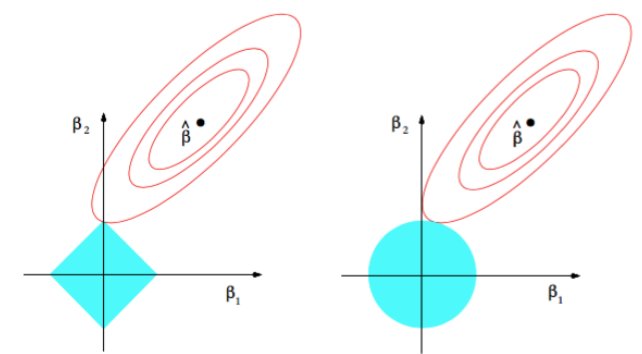
\includegraphics[width=5in]{pic4.png}
  \centering
  \caption{Estimation picture of the lasso (left) and ridge regression (right) \citep{Friedman2001}.}
  \label{img4}
\end{figure}

The previous section introduced some literature that used different Total Variance, and also introduced some basic knowledge about convex optimization. The following section will introduce the problems we need to solve.

\section{Problem Statement}

The goal of this article is to implement a real TV denoising algorithm from the python code step by step. For any picture, it can be shown as $X \in R_{n\times n}$. However, sparsity is not an inherent property of pictures, so we need a way to express the sparsity of pictures. Obviously, the difference between a pixel in the picture and the surrounding pixels can indicate whether this pixel is conspicuous in the picture. However, the noise of the picture will often produce many conspicuous points, which will affect the clarity of the picture.

Therefore, in order to eliminate noise, we need to propose a method to represent the number and intensity of the noise point in the image. This method is using the total variation (TV). For picture X, its TV is written as below.
$$
\|X\|_{T V}=\sum_{i=1}^{n-1} \sum_{j=1}^{n-1} \sqrt{\left(X_{i, j}-X_{i+1, j}\right)^{2}+\left(X_{i, j}-X_{i, j+1}\right)^{2}}\ \\
or\\
 \ \|X\|_{T V}=\sum_{i=1}^{n-1} \sum_{j=1}^{n-1}\left|x_{l, j}-X_{i+1, j}\right|+\left|X_{i, j}-X_{i, j+1}\right|
$$
Which of these two formulas is better? The two adjacent stores in the first formula are coupled together, which means that these two items cannot be handled separately. This leads to optimization difficulties. However, the two terms in the second formula are separate, which means that the two terms can be handled separately. From this perspective, the second method is more convenient. However, in fact, the adjacent points in the picture are coupled together, so using the first method will get better results. So we decided to use the left formula as part of our TV denoising algorithm.

Could it be possible that reducing the total variation help reduce noise? Through the above analysis, we know that the answer is yes. But if you do not set a limit, and directly reduce the total variation, it will cause other hard problems, such as the required details are eliminated and the sharp edges of the original become blurred. So in our optimization process, we will need an item so that the difference between denoised image and Noisy image is not too large. So a new variable is introduced to this problem.

$$
dissimilarity = \|F-X\|_{2}^{2}
$$
By minimize this term, we can make the denoised image and Noisy image similar to each other.

Finally, our optimization problem becomes the following form:

$$
\min _{X} \lambda\|X\|_{T V}+\|F-X\|_{2}^{2}
$$
In the following part of this article, the main task is to achieve an optimized solution to this problem through Python programming.


\section{Total Variance in Image denoising}

In this section, the complete derivation process of the image denoising algorithm will be introduced. To make the start simpler to understand, we choose the general gradient descent (GD) algorithm as the first step of denoising.

As stated in the previous section, our aim is to

$$
\min _{X} \lambda\|X\|_{T V}+\|F-X\|_{2}^{2}.
$$

According to the gradient descent algorithm, the problem can be solved with the following procedures:

\begin{algorithm}
\caption{Gradient Descent Algorithm}\label{alg1}
\begin{algorithmic}
\Procedure{Gradient Descent Algorithm with exact search}{}
\BState \emph{given} a starting point $x \in \operatorname{dom} f$ 
\BState \emph{repeat}:
\State 1. $\Delta x:=-\nabla f(x)$
\State 2. Line search. Choose step size $t$ via exact or backtracking line search.
\State 3. Update. $x:=x+t \Delta x$ 
\BState \emph{until} stopping criterion is satisfied.
\EndProcedure
\end{algorithmic}
\end{algorithm}

So it's needed to compute $\Delta x:=-\nabla f(x)$ every step, then we need to do exact line search in the direction of the negative side of the gradient.

\subsection{Calculate the gradient of the aim function}

In this section, the procedure of calculating the partial differentiation. Both of the following two items will be partially differentiated separately.

$$
\|X\|_{T V}=\sum_{i=1}^{n-1} \sum_{j=1}^{n-1} \sqrt{\left(X_{i, j}-X_{i+1, j}\right)^{2}+\left(X_{i, j}-X_{i, j+1}\right)^{2}}\
$$


$$
dissimilarity = \|F-X\|_{2}^{2}
$$

In the following subsections, the full procedures will be implemented.



\subsubsection{Calculate the partial differentiation of $\|X\|_{T V}$}



The condition of the related blocks is shown in figure \ref{img5}. According to the differential equation of the equation of TV, for every $x_{i,j}$, there will be three part of equations connected with it, and they are

\begin{equation*}%加*表示不对公式编号
\begin{split}
&\sqrt{\left(X_{i, j}-X_{i+1, j}\right)^{2}+\left(X_{i, j}-X_{i, j+1}\right)^{2}},\ \\
&\sqrt{\left(X_{i-1, j}-X_{i, j}\right)^{2}+\left(X_{i-1, j}-X_{i-1, j+1}\right)^{2}},\ \\
&\sqrt{\left(X_{i, j-1}-X_{i+1, j-1}\right)^{2}+\left(X_{i, j-1}-X_{i, j}\right)^{2}},\
\end{split}
\end{equation*}


and as you can see, there will be three inverse “L” shape block hit the center block for every $x_{i,j}$, and each of them is colored with blue, green, and red.


\begin{figure}[h]
  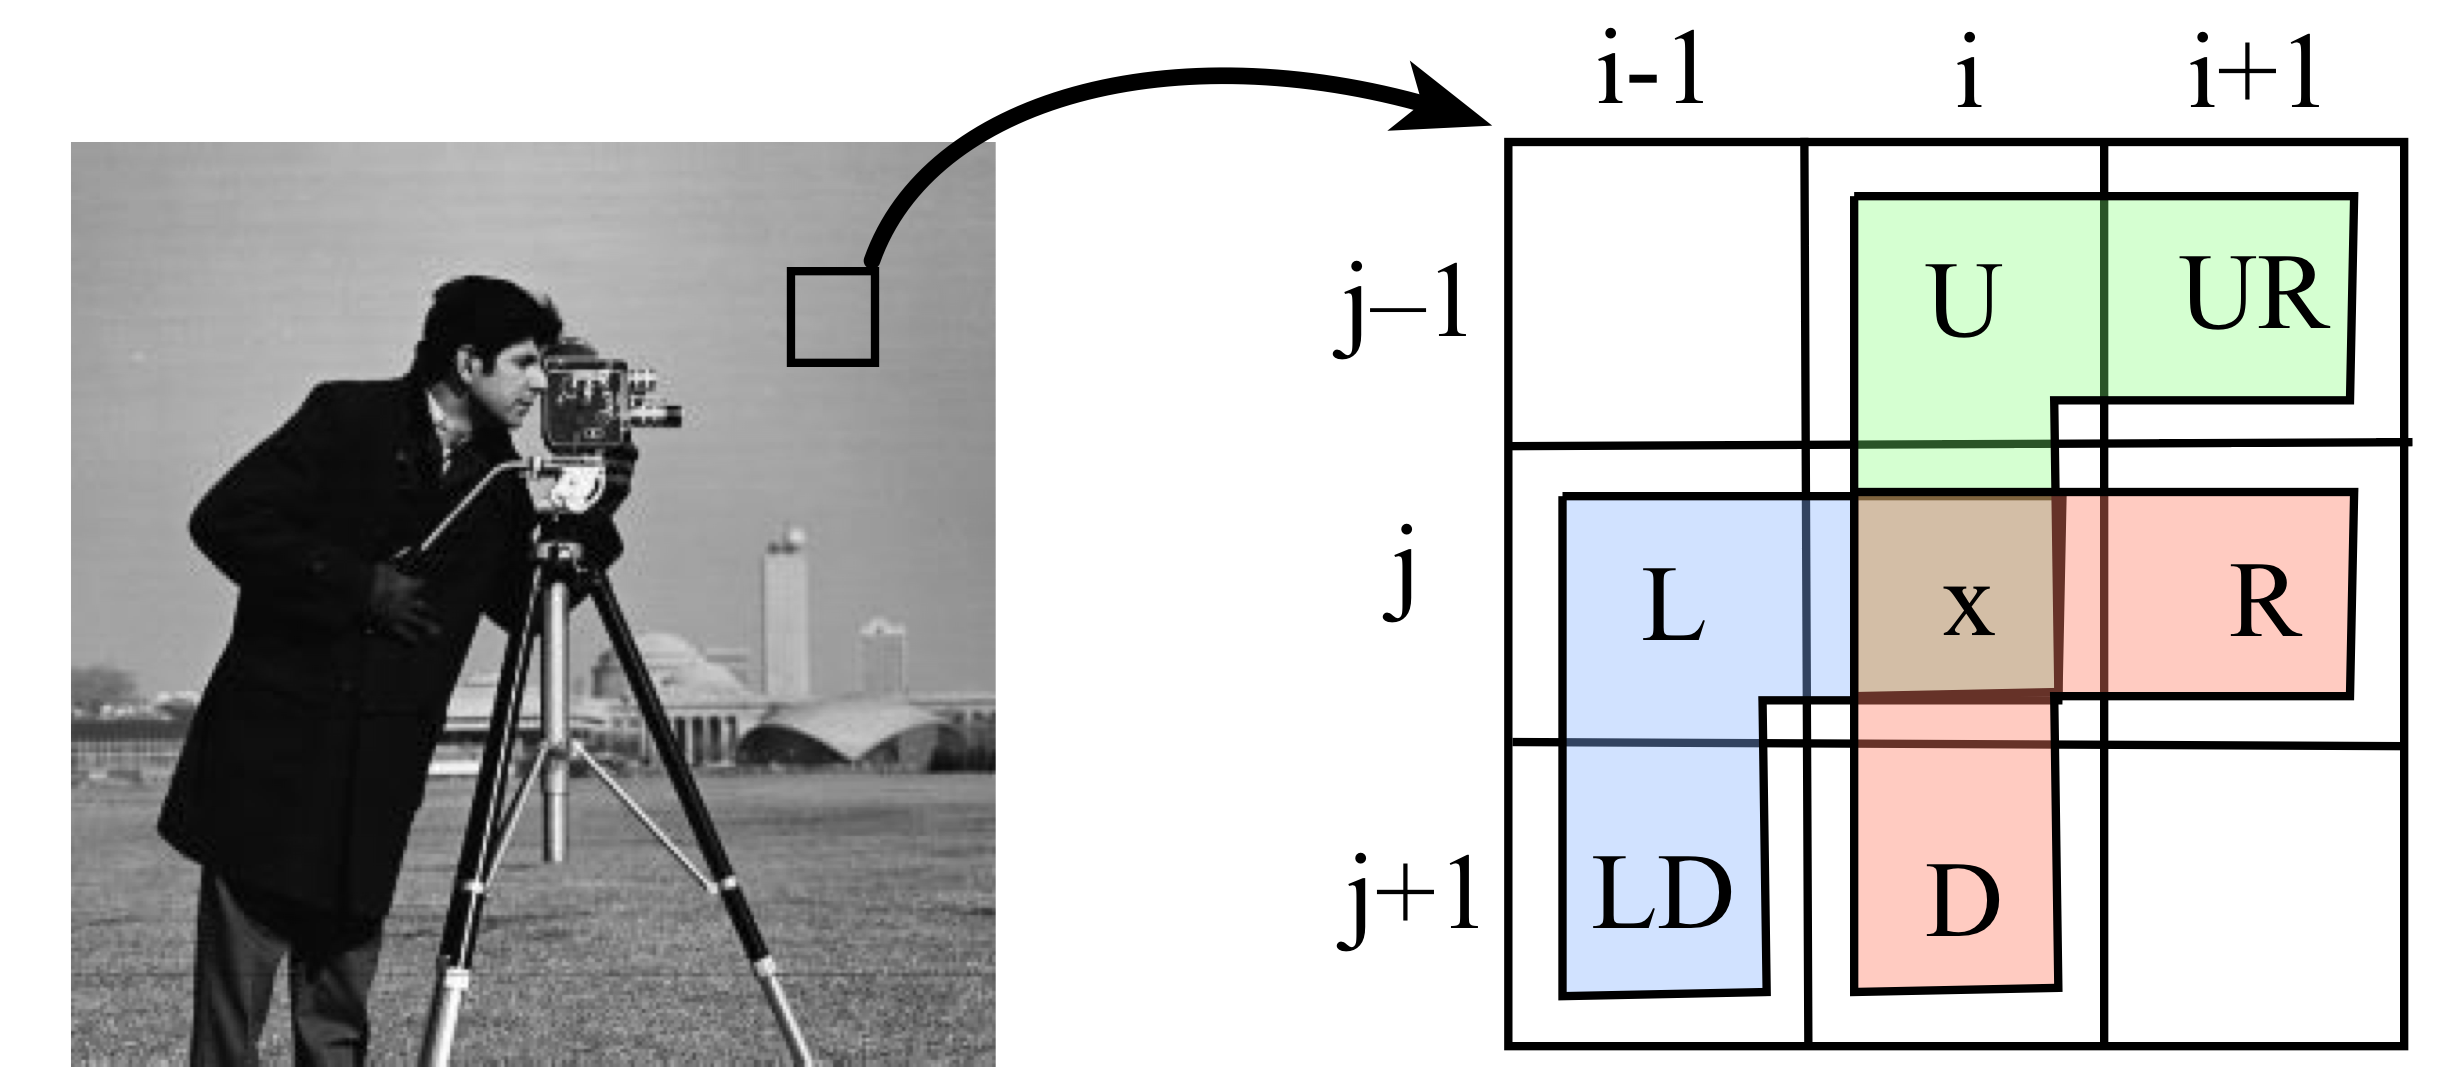
\includegraphics[width=3in]{pic5.png}
  \centering
  \caption{the representation of one center pixel surrounded by eight pixels.}
  \label{img5}
\end{figure}

By looking at the three equations connedted with $x_{i,j}$, it can be found that they can be seperated to to part, $\sqrt{(x-a)^{2}+(x-b)^{2}}$ and $\sqrt{(a-x)^{2}+(a-b)^{2}}$. To Calculate $\frac{\partial}{\partial x}\|X\|_{T V}$, the partial diffrenciation of these two equation should be calculated first.



$$
\frac{\partial}{\partial x}(\sqrt{(x-a)^{2}+(x-b)^{2}})= 
\frac{-a-b+2 x}{\sqrt{a^{2}-2 a x+b^{2}-2 b x+2 x^{2}}}
$$

$$
\frac{\partial}{\partial x}(\sqrt{(a-x)^{2}+(a-b)^{2}})=-\frac{a-x}{\sqrt{(a-b)^{2}+(a-x)^{2}}}
$$

The Python implecation of these equations are shown below:

\begin{python}
def delTV(L, R, U, D, LD, UR, x):
    def delTV1(a,b,x):
        divider = a*a - 2*a*x + b*b - 2*b*x + 2*x*x
        return (-a-b+2*x)/math.sqrt(divider) if divider>0 else 0
    def delTV2(a,b,x):
        divider = math.sqrt((a-b)*(a-b)+(a-x)*(a-x))
        return (-a+x)/divider if divider>0 else 0
    return delTV1(D, R, x) + delTV2(L,LD,x) + delTV2(U,UR,x)
\end{python}


\subsubsection{Calculate the partial differentiation of $\|F-X\|_{2}^{2}$}

For this part, it can be solved easily.

$$
\frac{\partial}{\partial x}\left((a-x)^{2}\right)=2 x-2 a
$$


\subsection{Deal with the boundary condition}

After implementing all the cells inside the image, there comes a problem that when meeting with the boundary, all these equations will lose some information as shown in figure \ref{img6}. For the shadow part, they are the missing message.

\begin{figure}[h]
  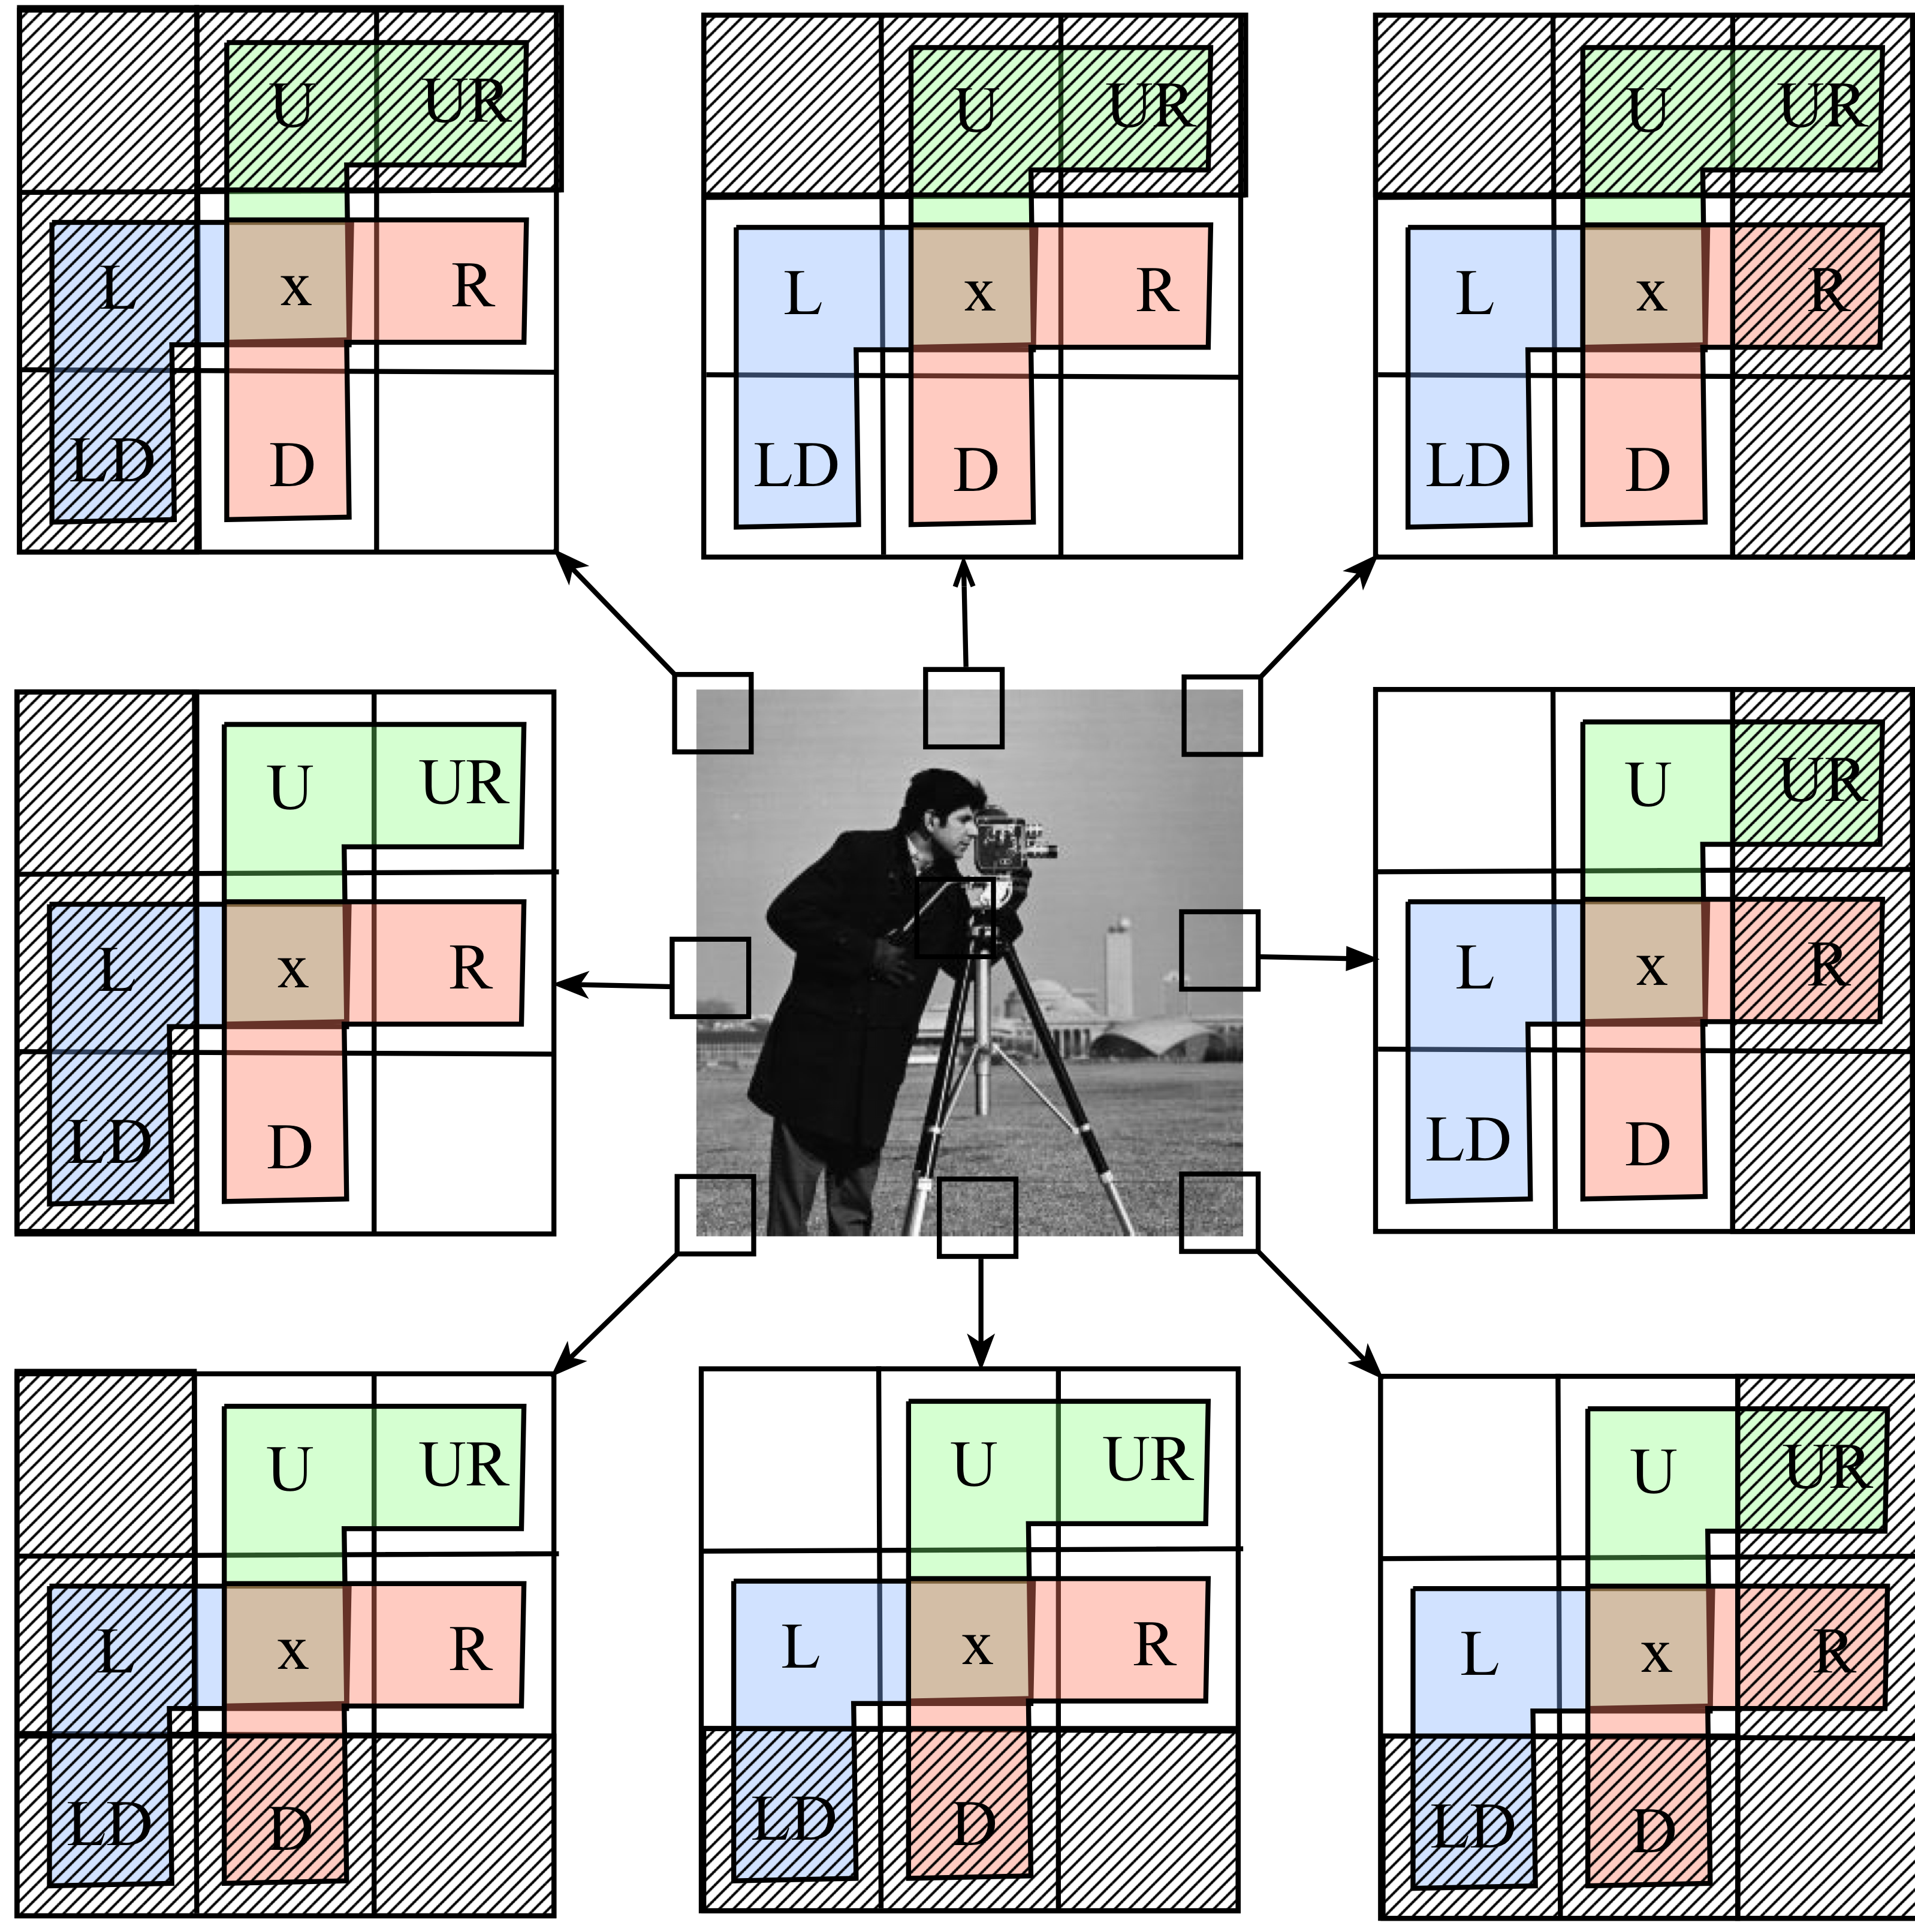
\includegraphics[width=3.5in]{pic6.png}
  \centering
  \caption{The boundary condition for the sample image which is hard to solve.}
  \label{img6}
\end{figure}


It’s not easy to deal with this problem, and for the current state, ignoring the boundary pixels is one choice. This problem will be solved in future updates.

\subsection{Implement the Gradient Descent for Total Variation Denoising}

In the folder of code, \textit{GD-general.ipynb} and \textit{GD-general.py} can be found (the content of them is the same). In the inner folder img, some original images can be seen, and they are downloaded from \textit{https://www.math.ust.hk/~masyleung/Teaching/CAS/MATLAB/image/target2.html}. After running \textit{GD-general.ipynb}, the output files are saved in the inner folder \textit{gen-img}, and the example of the denoising processing are shown in figure \ref{img7}. The Noised images are generated with Gauss Noise (GN). The algorithm of Gauss Noise is in img.py.

\begin{python}
    def gaussNoise(im_array, sigma):
        im_array_flat = im_array.flatten()
        for i in range(im_array.shape[0]*im_array.shape[1]):
            pointInFlat = int(im_array_flat[i])+ random.gauss(0,sigma)
            if pointInFlat < 0:
                pointInFlat = 0
            if pointInFlat > 255:
                pointInFlat = 255
            im_array_flat[i] = pointInFlat
        im_array = im_array_flat.reshape([im_array.shape[0],im_array.shape[1]])
        return im_array
\end{python}


As shown in figure \ref{img7}, the leftmost one is the original image directly downloaded from the website, and the next one is the noised image. Then the following three images are the denoised image with iteration 1, 10, and 100. It can be found that after 10 iterations, the noised image is already much better than the first iteration.

\begin{figure}[h]
  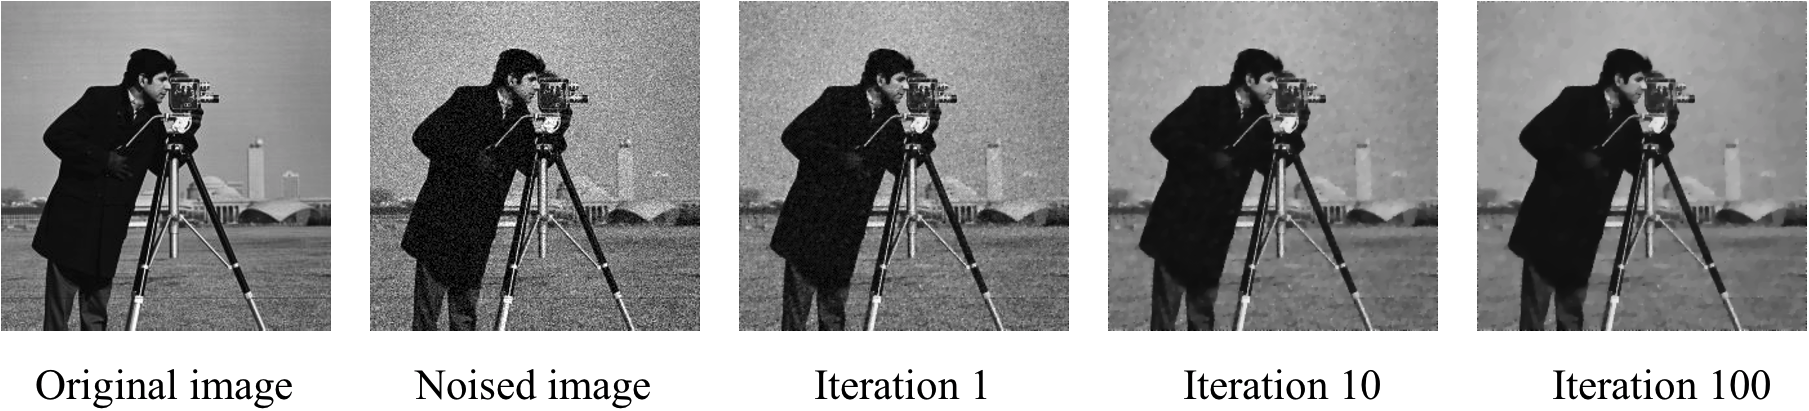
\includegraphics[width=5in]{./pic7.png}
  \centering
  \caption{The original image, noised image, and three images are the denoised image with iteration 1, 10, and 100 with gradient descent.}
  \label{img7}
\end{figure}

To show the speed of convergence, $f(x^{k})$ vs. time and  $f(x^{k})$ vs. iteration k are shown in figure \ref{img8} and figure \ref{img9}. It can be found that at first iterations, the speed of convergence is fast. However, after some iterations, the speed is much slower.

\begin{figure}[h]
  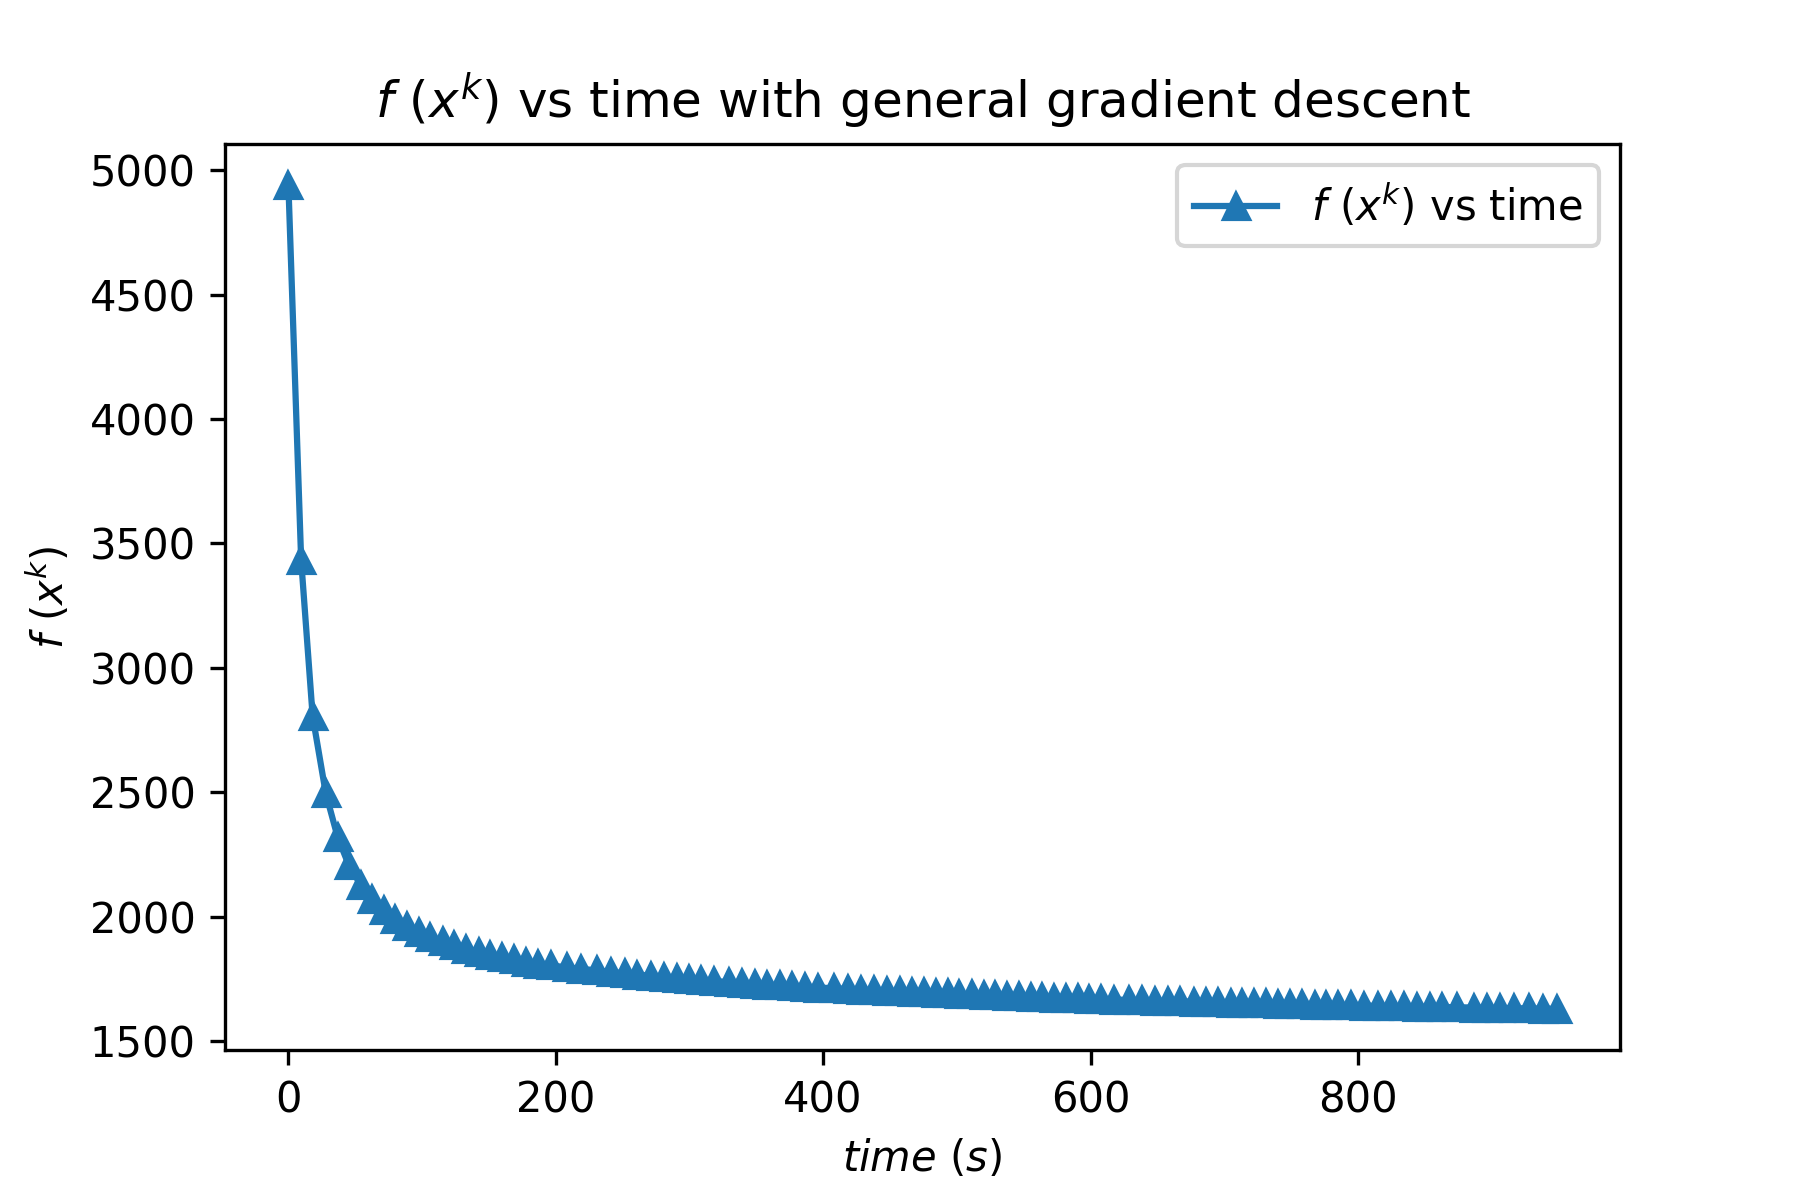
\includegraphics[width=3.5in]{pic8.png}
  \centering
  \caption{$f(x^{k})$ vs. time for general gradient discent.}
  \label{img8}
\end{figure}

\begin{figure}[h]
  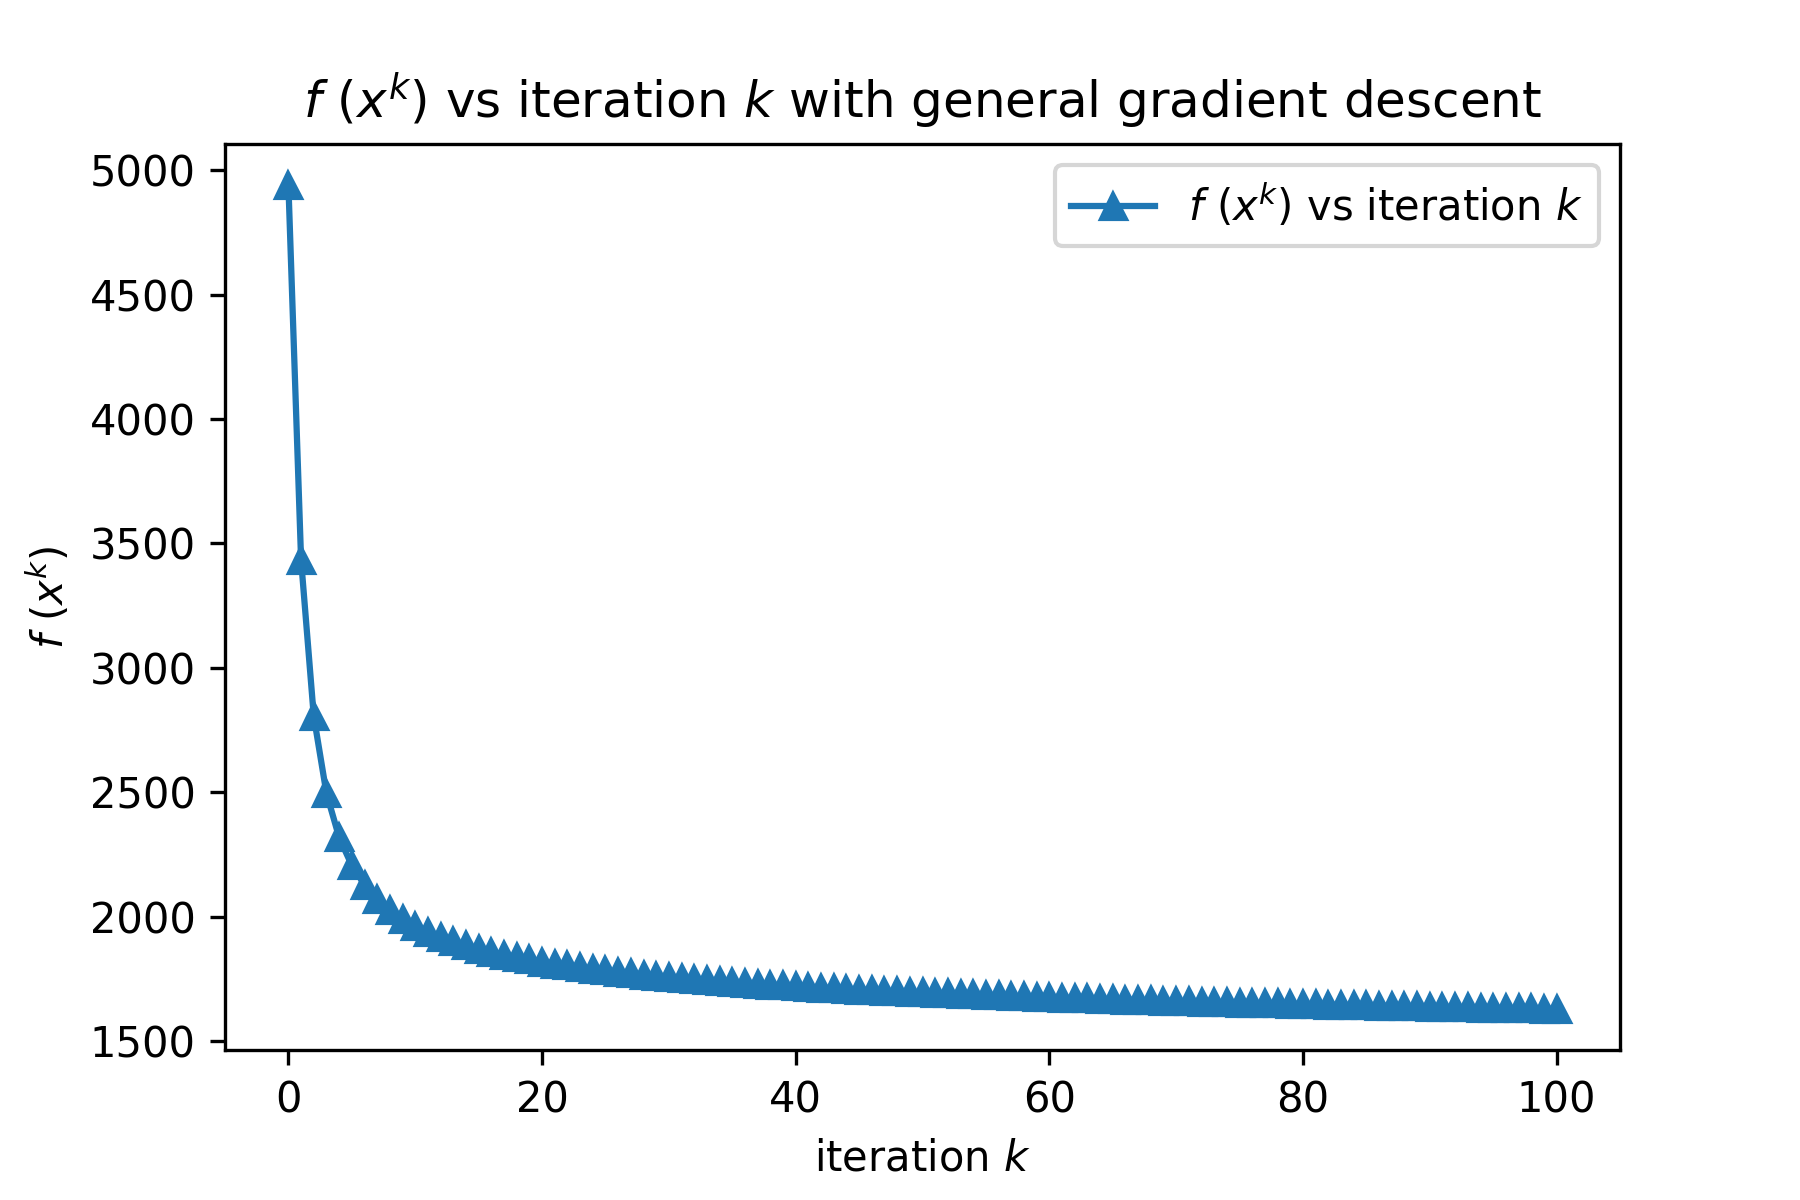
\includegraphics[width=3.5in]{pic9.png}
  \centering
  \caption{$f(x^{k})$ vs. iterration k for general gradient discent.}
  \label{img9}
\end{figure}

\section{Optimization of the TV algorithm}

\subsection{Implement the Nesterov Acceleration to Accelerate Gradient Descent}

To accelerate the speed of convergence, Nesterov acceleration is chosen as the speed-up algorithm. And the thinking of methods is shown below.

$$
\begin{array}{l}
z_{k+1}=x_{k}-t_{k} \nabla f\left(x_{k}\right) \\
x_{k+1}=z_{k+1}+\delta_{k}\left(z_{k+1}-z_{k}\right) \quad \delta_{k} \in[0,1)
\end{array}
$$

And the algorithm is shown below \citep{Ioannis2018}.

\begin{algorithm}
\caption{Gradient Descent Algorithm}\label{alg1}
\begin{algorithmic}
\Procedure{Gradient Descent Algorithm with Nesterov Acceleration }{}
\BState \emph{given} a starting point $x \in \operatorname{dom} f$, learning rate $\delta_{k}$
\BState \emph{repeat}:
\State 1. $z_{k+1}=x_{k}-t_{k} \nabla f\left(x_{k}\right)$
\State 2. $x_{k+1}=z_{k+1}+\delta_{k}\left(z_{k+1}-z_{k}\right) \quad \delta_{k} \in[0,1)$
\State 3. Line search. Choose step size $t$ via exact or backtracking line search.
\State 4. Update. $x:=x_{k+1}(t_{k})$ 
\BState \emph{until} stopping criterion is satisfied.
\EndProcedure
\end{algorithmic}
\end{algorithm}

\citet{Ioannis2018} also Compared Polyak’s method with Nesterov’s algorithm. Ioannis says that Polyak’s method evaluates the gradient before adding momentum, while Nesterov’s algorithm evaluates the gradient after applying momentum as shown in figure \ref{img10} \citep{Ioannis2018}.

\begin{figure}[h]
  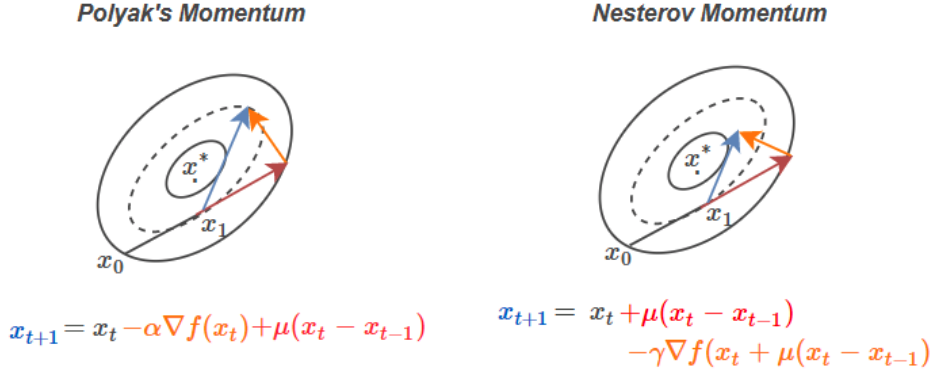
\includegraphics[width=4.5in]{pic10.png}
  \centering
  \caption{Comparison of Polyak’s method and Nesterov’s algorithm.}
  \label{img10}
\end{figure}

Just applying this method, the output is very similar to the pure exact gradient search (figure \ref{img11}). But the difference is not easy to be seen by human eyes. So the $f(x^{k})$ vs. time and  $f(x^{k})$ vs. iteration k are presented to show the speed of convergence, in figure \ref{img12} and figure \ref{img13}. It can be found that at first iterations, the speed of convergence is fast. However, after some iterations, the speed is much slower.

\begin{figure}[h]
  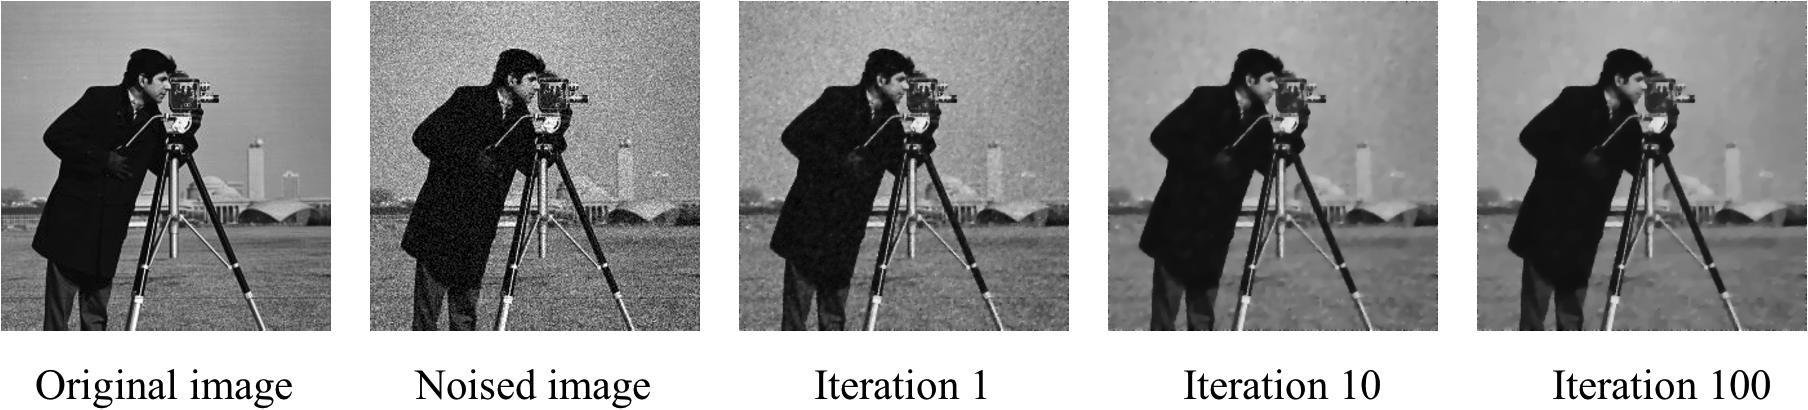
\includegraphics[width=5in]{pic11.png}
  \centering
  \caption{The original image, noised image, and three images are the denoised image with iteration 1, 10, and 100 with gradient descent accelerated by the Nesterov method.}
  \label{img11}
\end{figure}

\begin{figure}[h]
  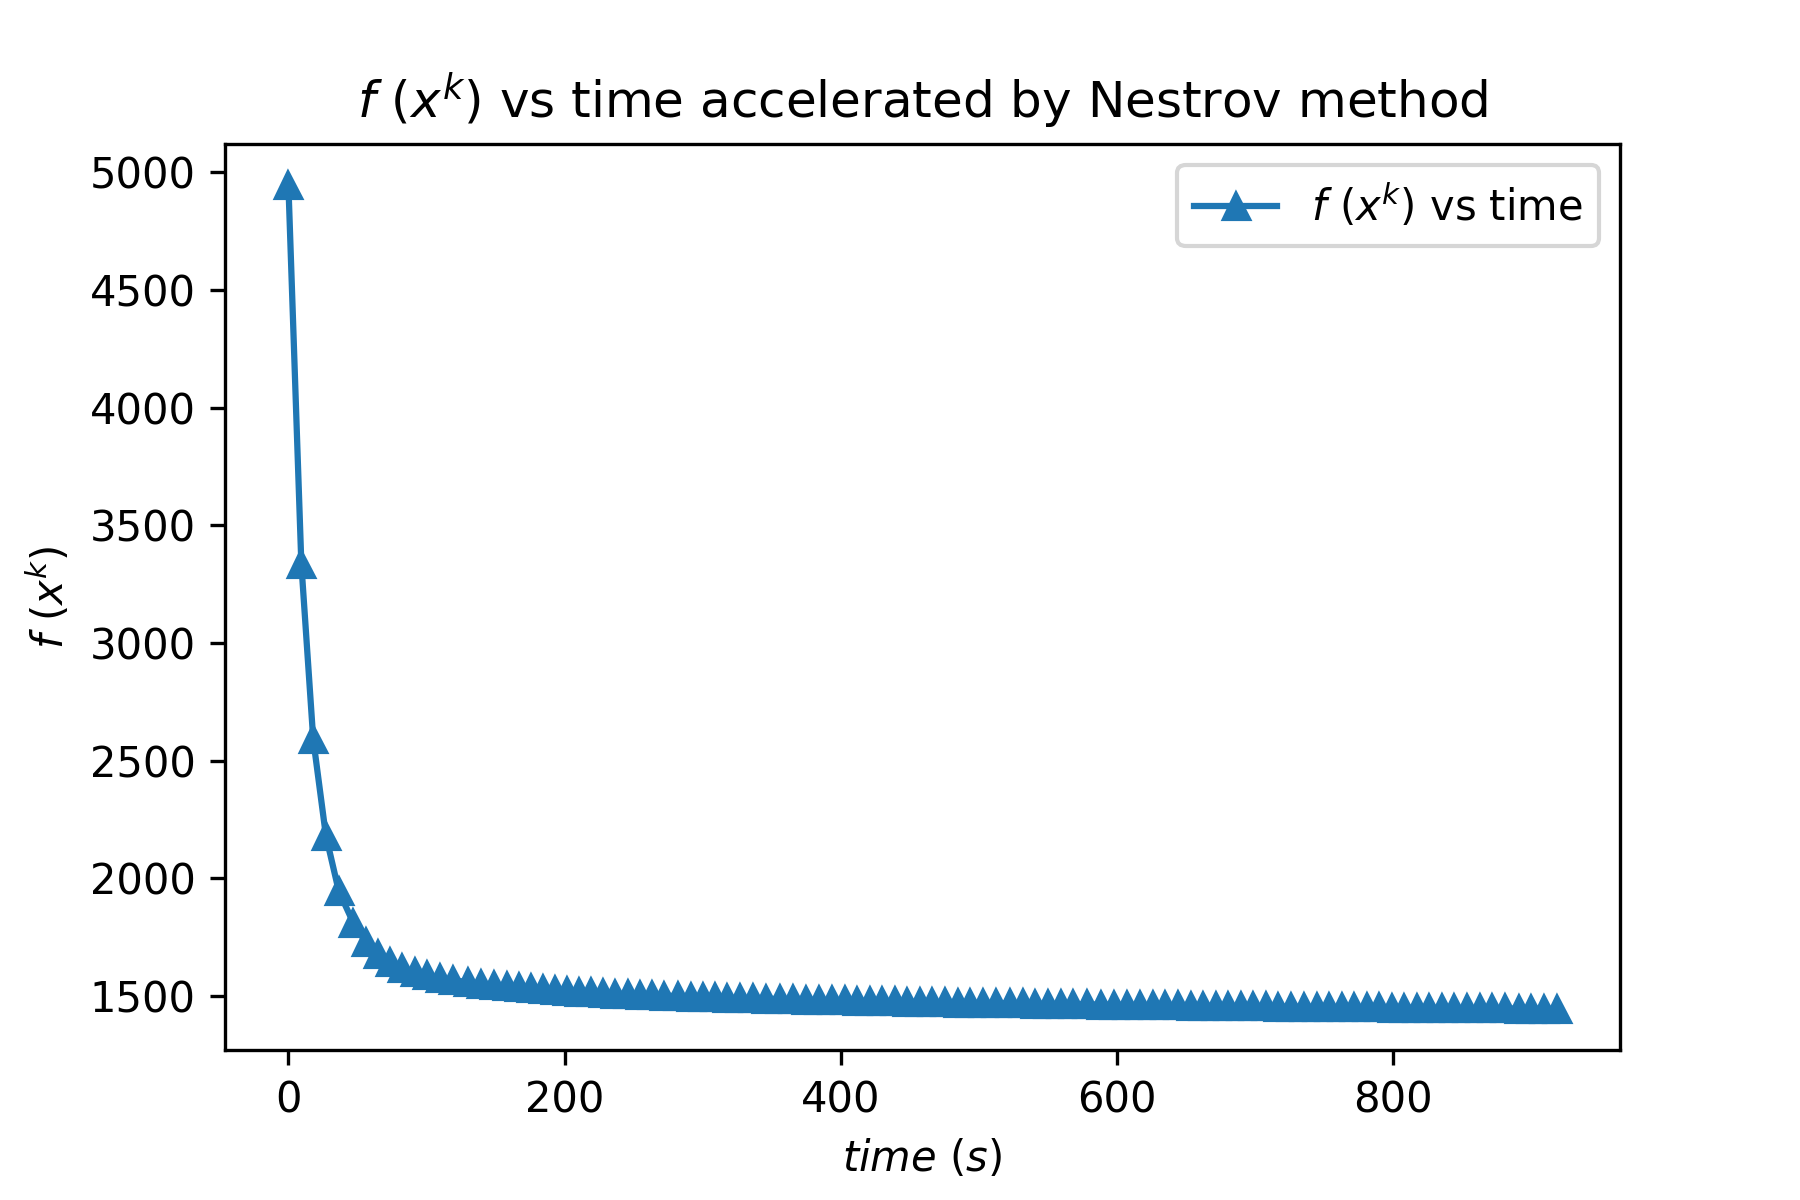
\includegraphics[width=3.5in]{pic12.png}
  \centering
  \caption{$f(x^{k})$ vs. time for gradient discent accelerated by Nestrov method.}
  \label{img12}
\end{figure}

\begin{figure}[h]
  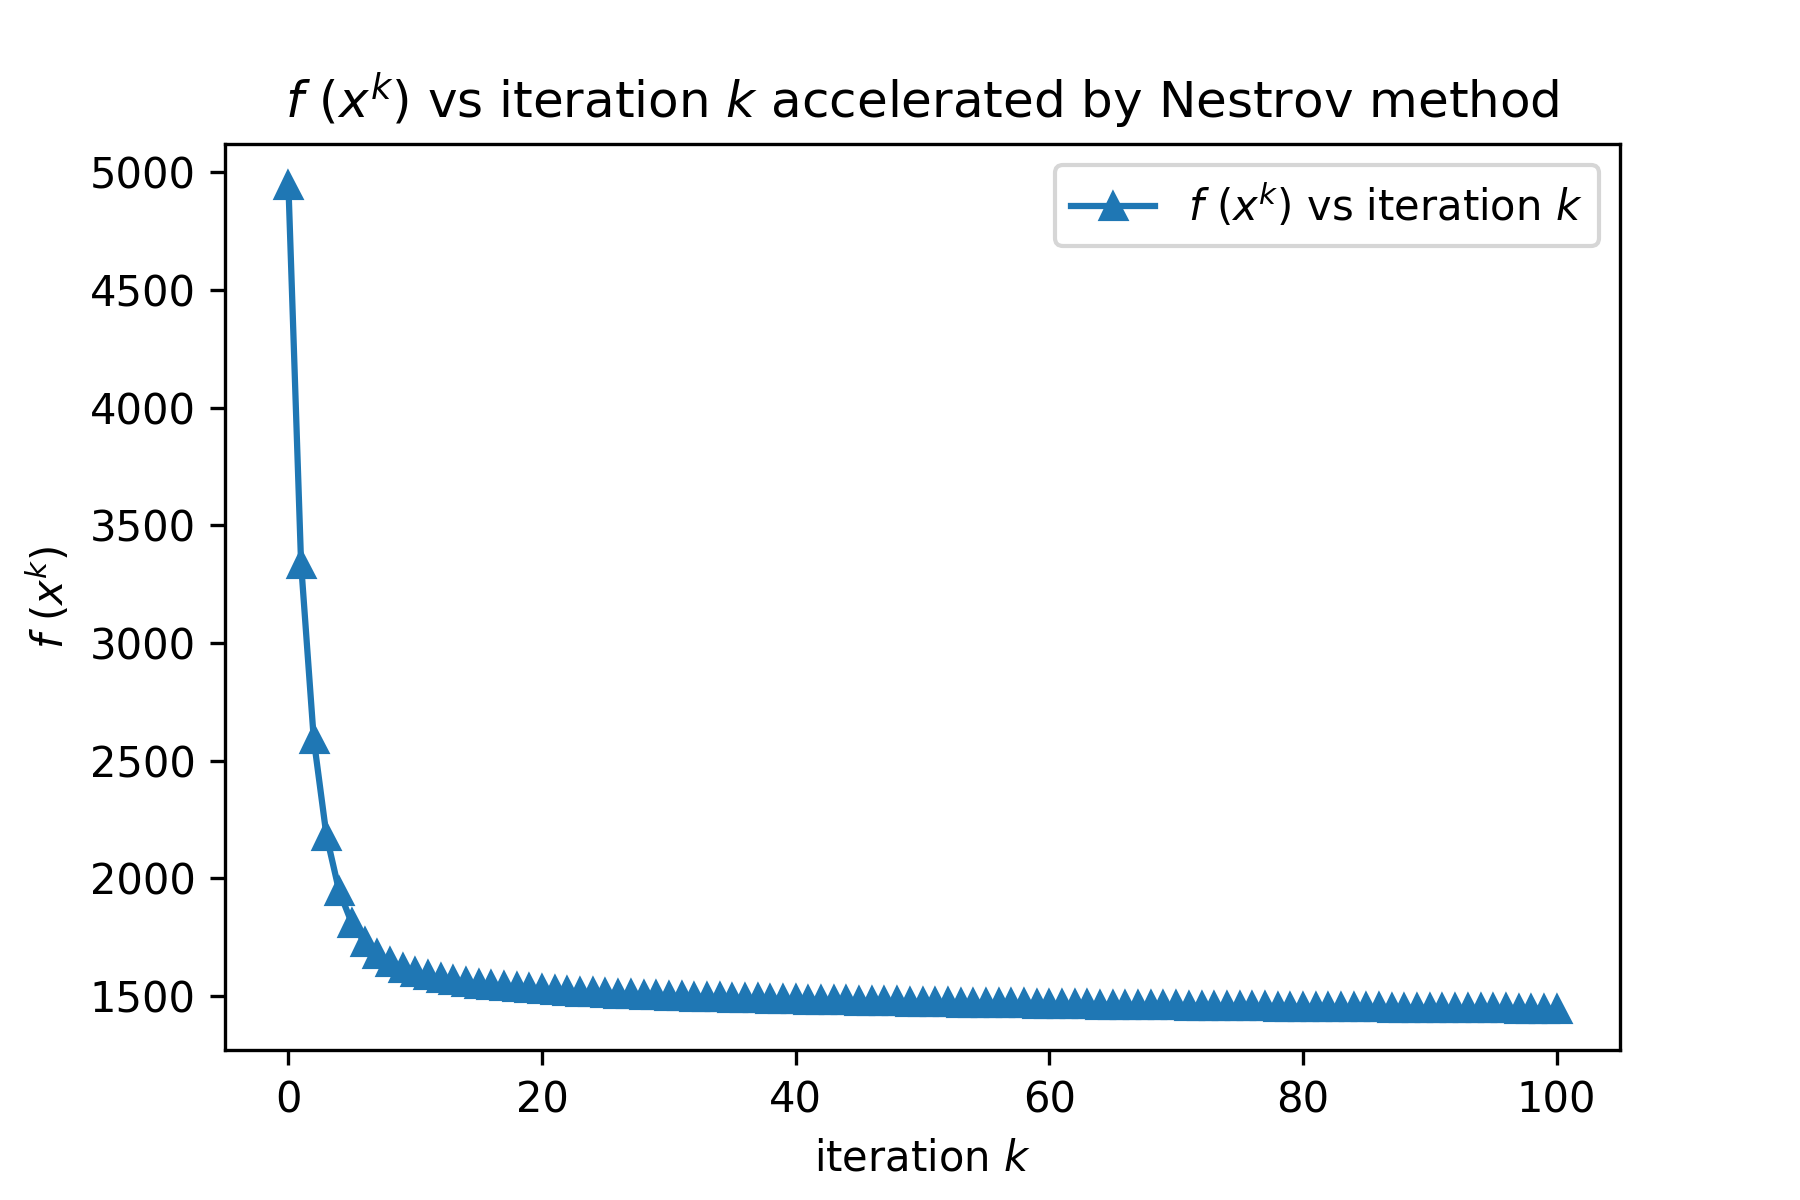
\includegraphics[width=3.5in]{pic13.png}
  \centering
  \caption{$f(x^{k})$ vs. iteration k for gradient discent accelerated by Nestrov method.}
  \label{img13}
\end{figure}



\subsection{Comparison of gradient descent and gradient descent accelerated by Nesterov method}

Still, comparing those graphs in one figure is a better way to show the difference. Figure \ref{img14} shows the comparison of $f(x^{k})$ vs. time for gradient descent and gradient descent accelerated by Nesterov method. 

When accelerated by the Nesterov method, it only cost 82 seconds to reach the value that general gradient descent needs to cost 918 seconds to reach, which is 10 times faster! 

Comparing $f(x^{k})$ vs. iteration for gradient descent and gradient descent accelerated by Nesterov method as figure \ref{img15} present the same output: Nesterov method only cost 9 iterations to reach the value that general gradient descent need to cost 100 iterations to reach, which is also about 10 times faster! 

\begin{figure}[h]
  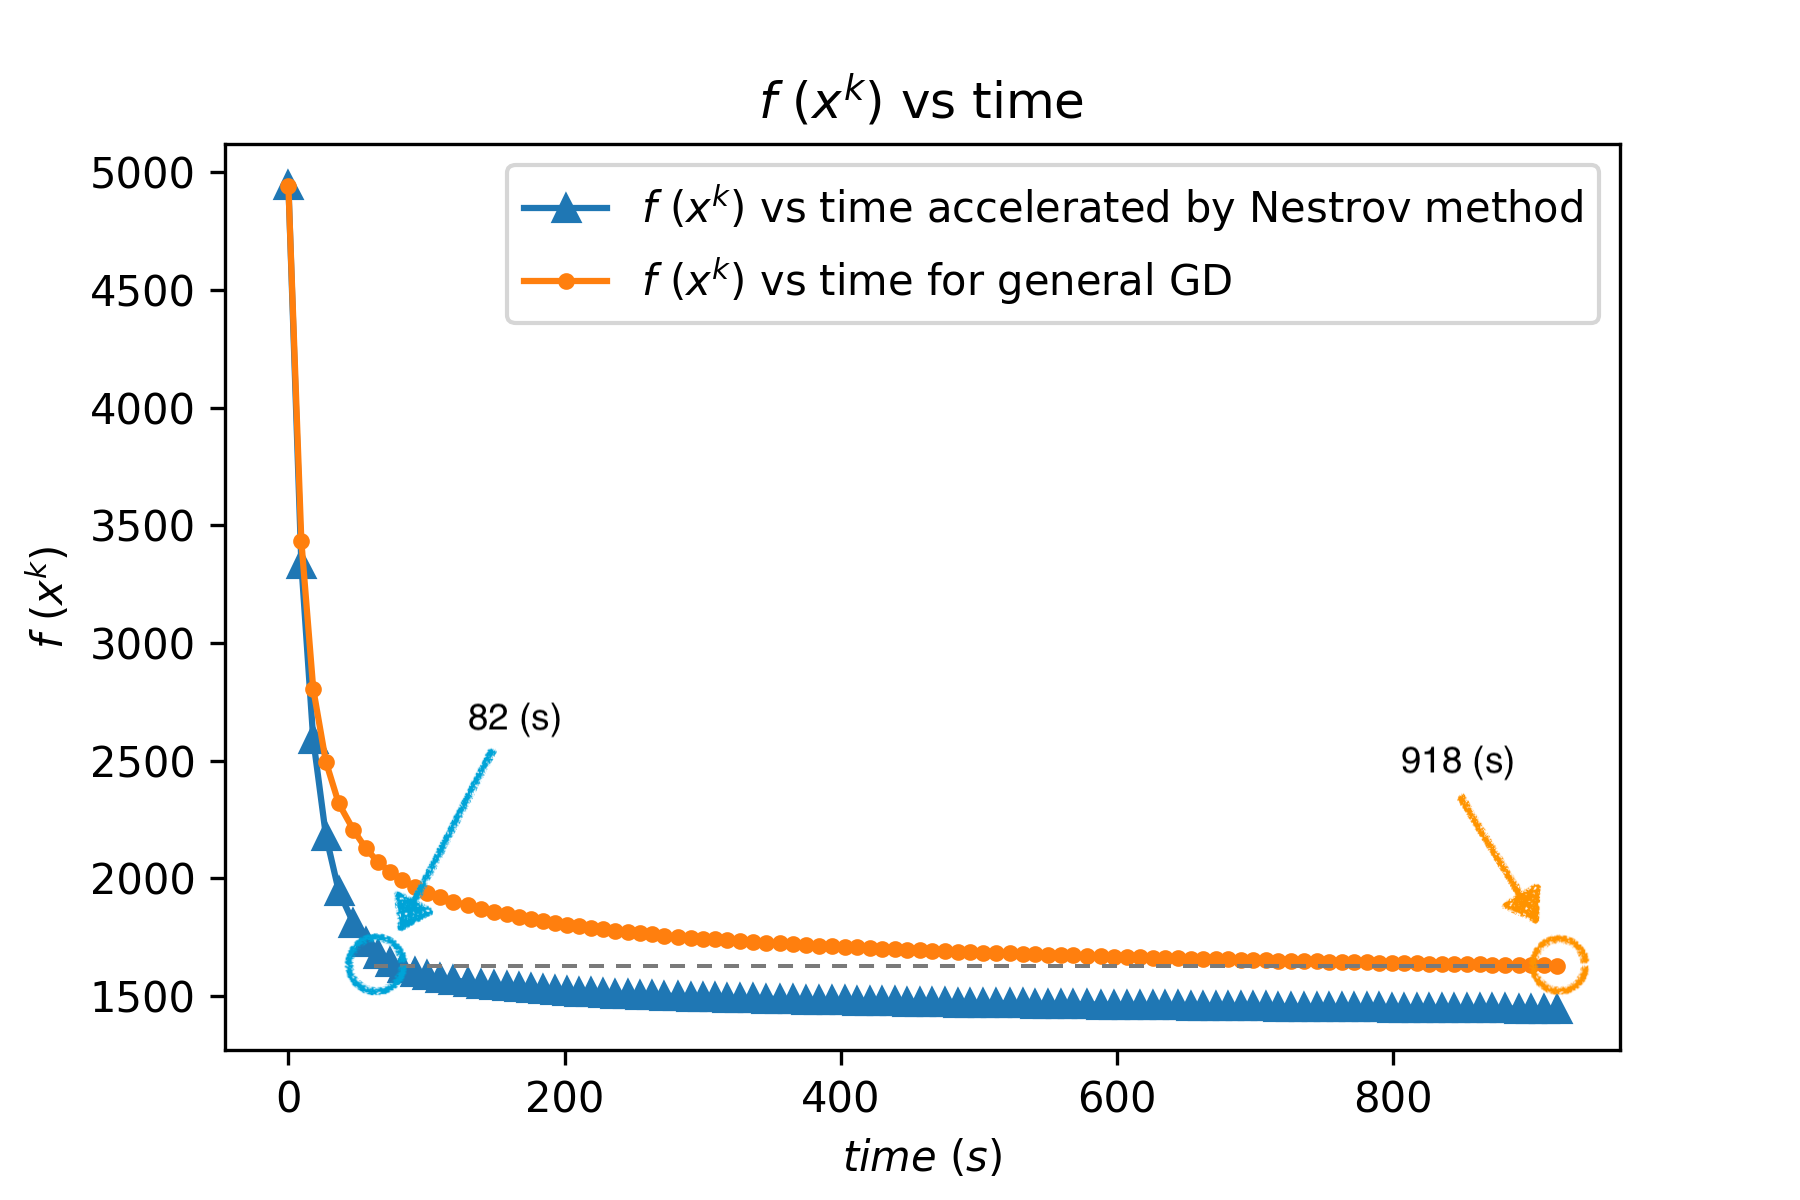
\includegraphics[width=3.5in]{pic14.png}
  \centering
  \caption{Comparision of $f(x^{k})$ vs. time for gradient descent and gradient descent accelerated by Nesterov method.}
  \label{img14}
\end{figure}

\begin{figure}[h]
  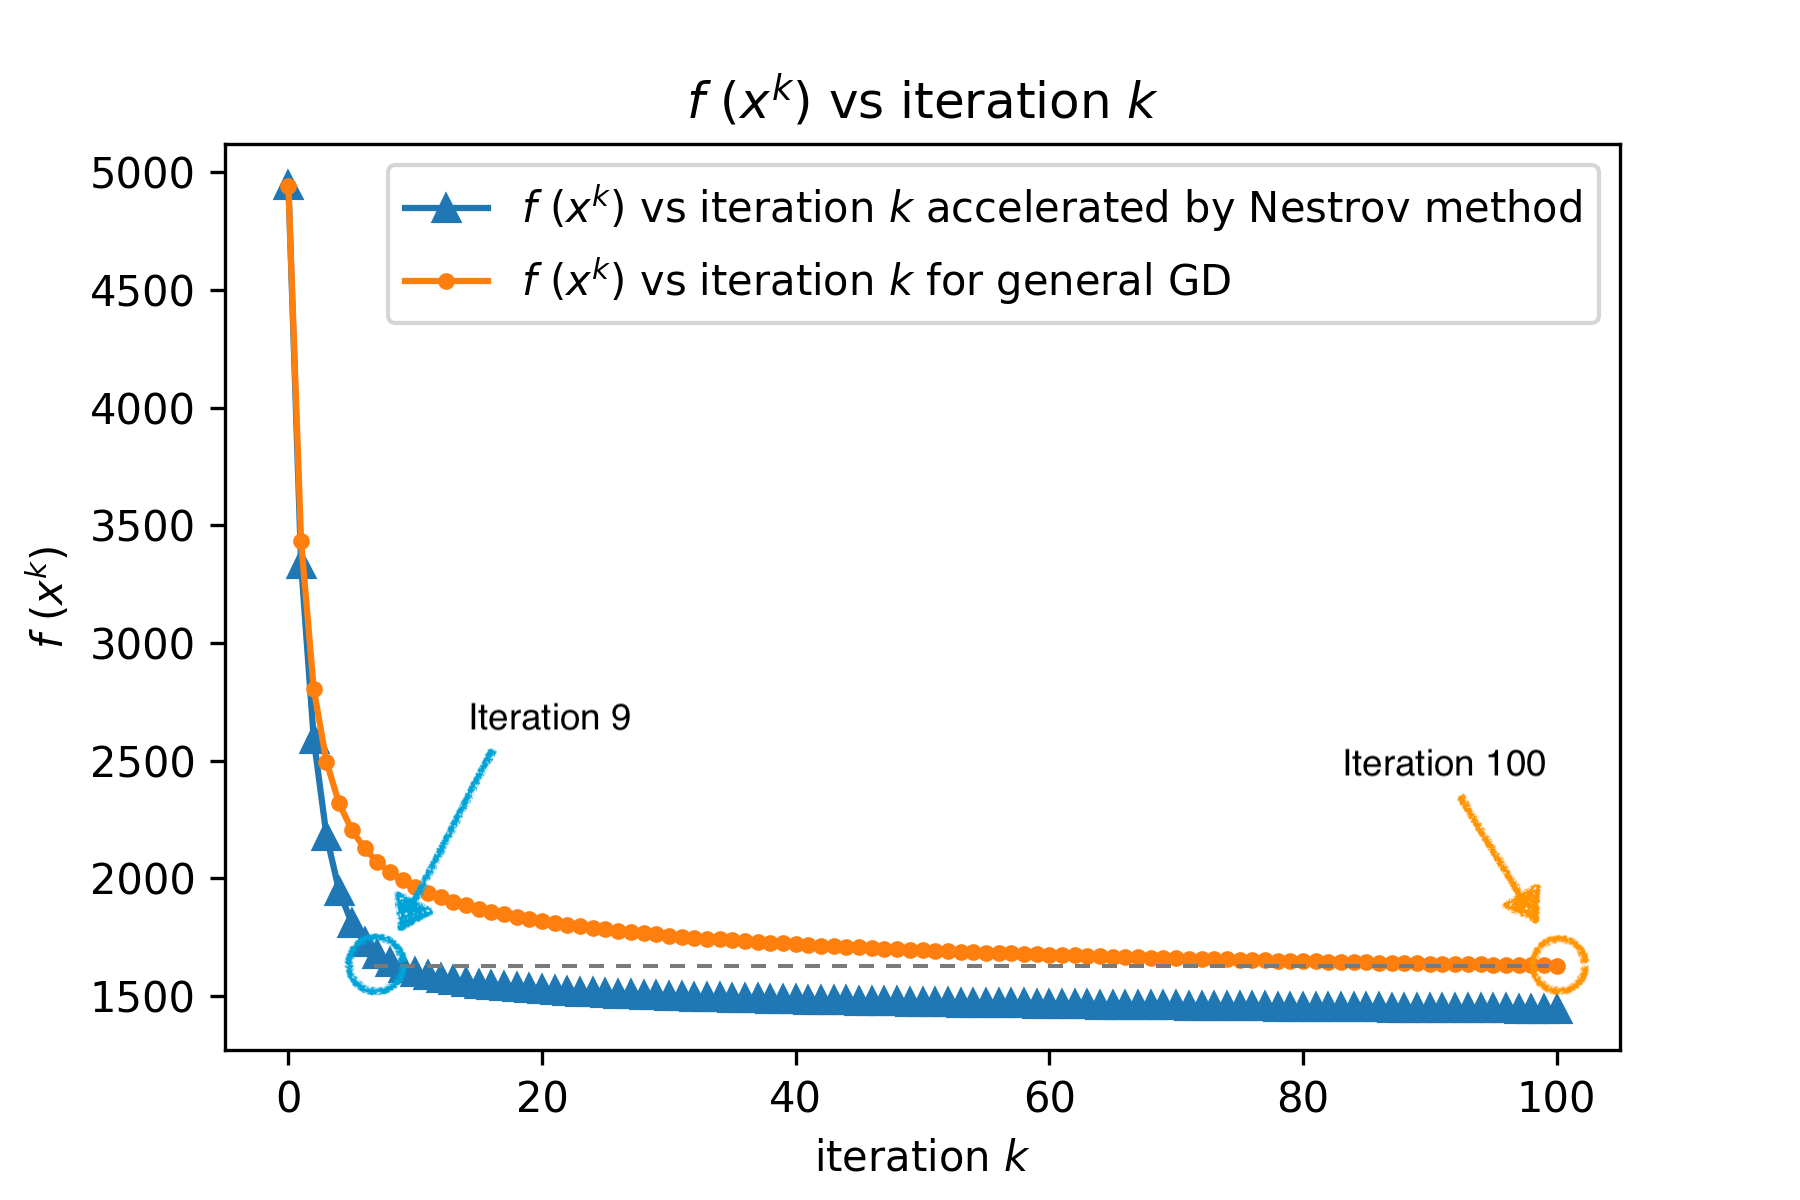
\includegraphics[width=3.5in]{pic15.png}
  \centering
  \caption{Comparision of $f(x^{k})$ vs. iteration k for gradient descent and gradient descent accelerated by Nesterov method.}
  \label{img15}
\end{figure}

\subsection{Implement the Stochastic Method to Accelerate Gradient Descent}

Because there are many pixels in one single image, it would be difficult to calculate the best descent direction, and for one direction, the step size would not be the best length for every pixel.

To make the selection of step size more efficient, it could be better to take apart the single image to multiple small images, and then do gradient descent for every small image separately.

A simple solution is to split an image to multiple n by n rectangles, and according to figure \ref{img5}, there should be a margin as a helper to calculate the differentiation of the center split images. 

To make the process simpler and easy to understand, we define one iteration as one full polling of all split blocks. And there will always process all blocks one by one with no multiprocess, which means in this case, the time would be the real time that needed to finish all the calculations without any trick.

First, let me to introduce you the $f(x^{k})$ vs. time and  $f(x^{k})$ vs. iteration k are presented to show the speed of convergence, in figure \ref{img16} and figure \ref{img17}, compared with the general gradient discent and the gradient discent accelarated by Nesterov method.

\begin{figure}[h]
  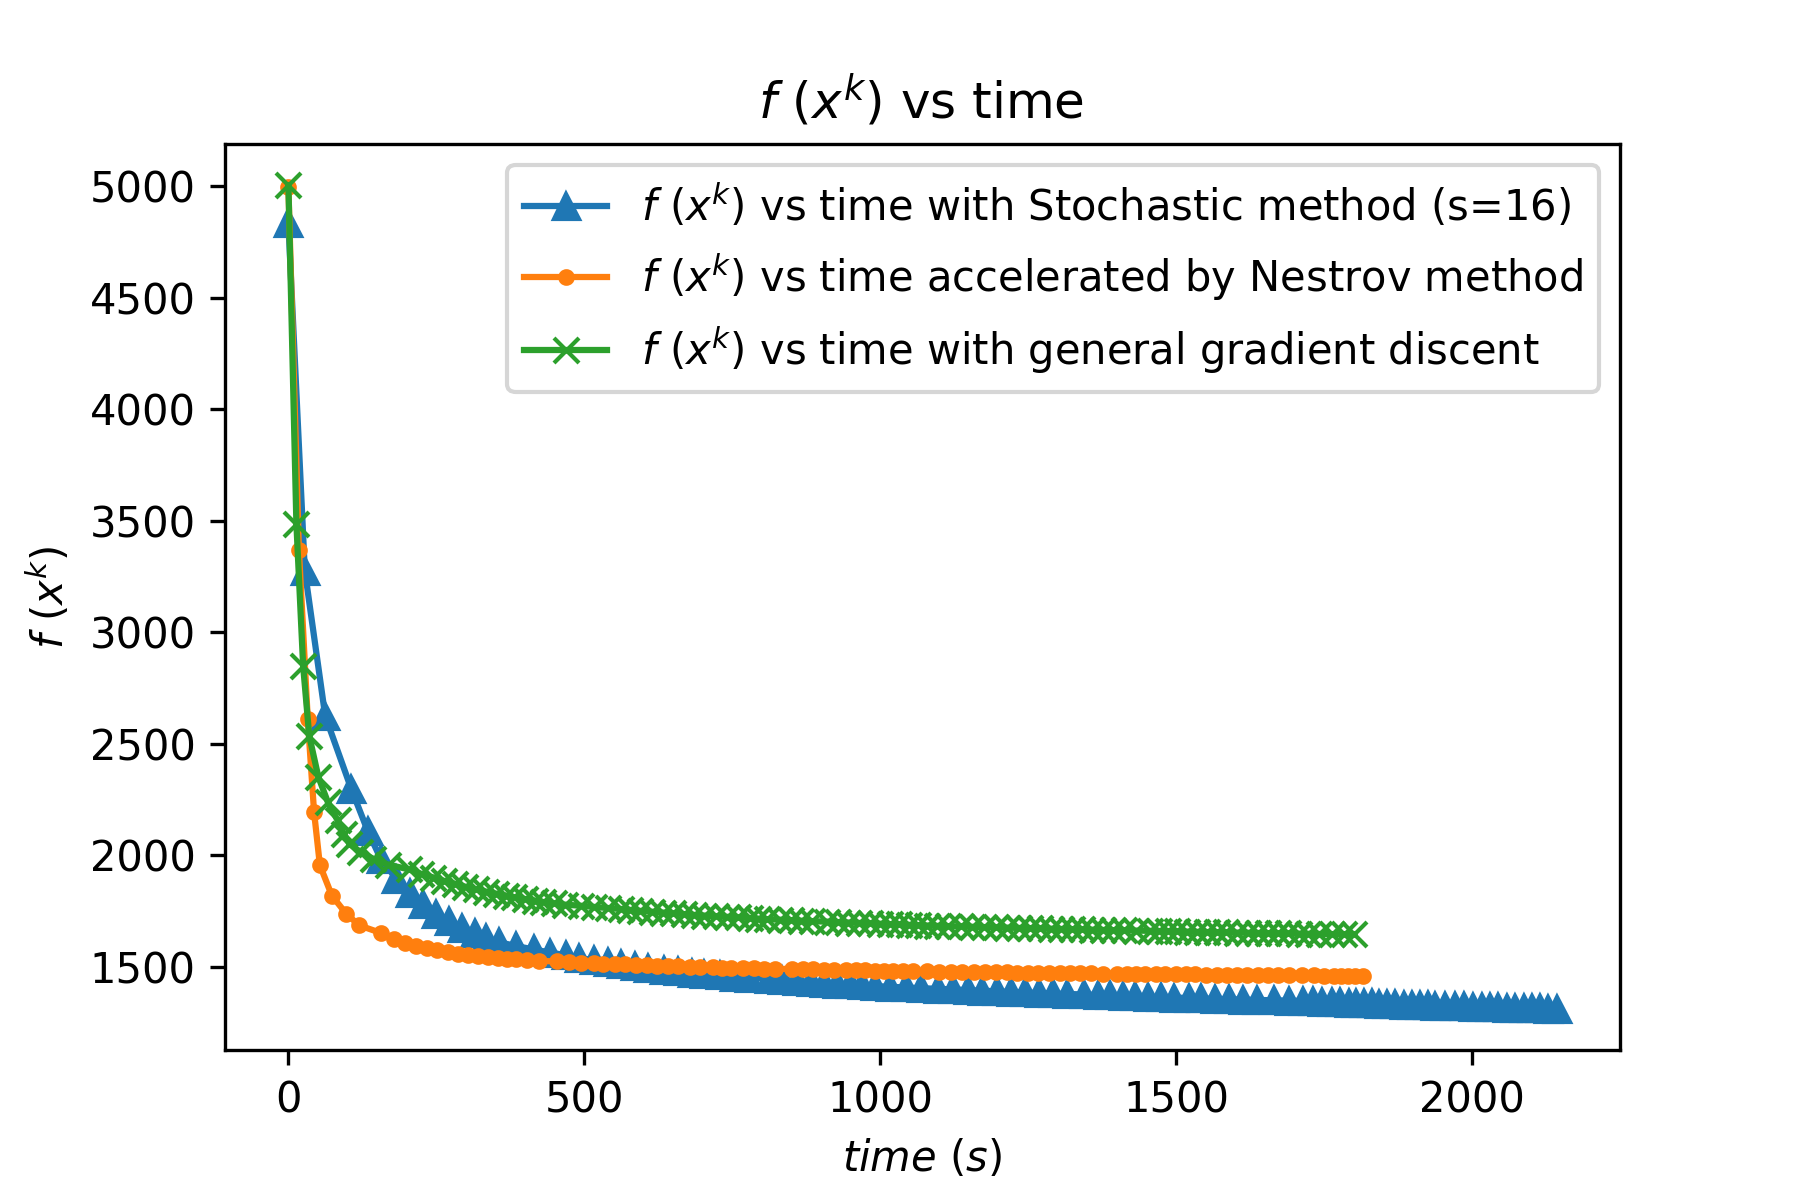
\includegraphics[width=3.5in]{pic16.png}
  \centering
  \caption{Comparision of $f(x^{k})$ vs. time for gradient descent, gradient descent accelerated by the Nesterov method, and gradient descent accelerated by the Stochastic method.}
  \label{img16}
\end{figure}

\begin{figure}[h]
  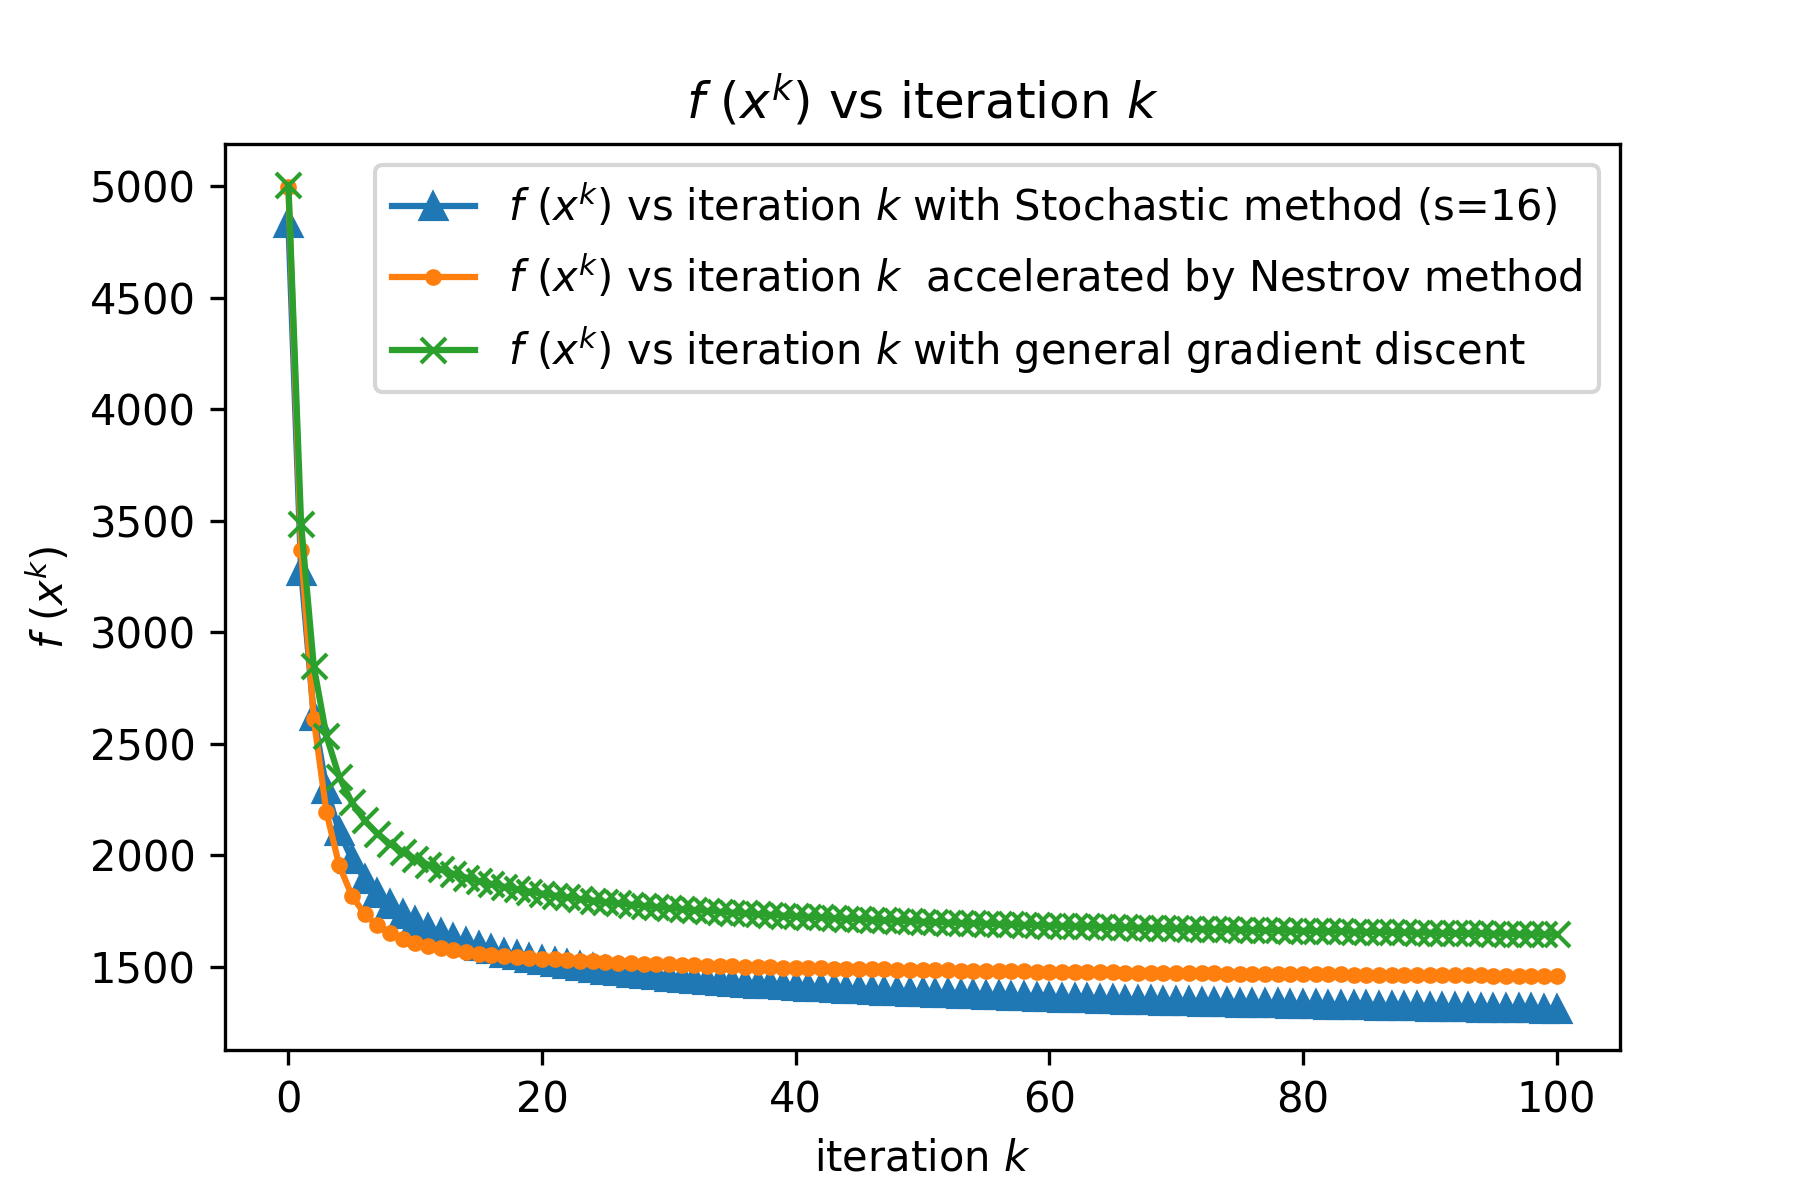
\includegraphics[width=3.5in]{pic17.png}
  \centering
  \caption{Comparision of $f(x^{k})$ vs. iteration k for gradient descent, gradient descent accelerated by the Nesterov method, and gradient descent accelerated by the Stochastic method.}
  \label{img17}
\end{figure}

As you can see in figure \ref{img16}, the overall time of 100 iterations for Gradient descent with the stochastic method is longer than the previous two methods, this is because there need to calculate the best step size with exact line search for $(k/n)^2$ times, where $k$ is the length of the image, and $n$ is the size of the block you choose. Though the calculation of the best step size is much more than the previous two solutions, it works better when time is long enough. This is because when some block with a low score has already reached its best state, there can be many other blocks that can be improved largely without being affected by those already converged blocks.

Considering figure \ref{img16}, we can get the same conclusion, but due to the inconsistency of the time and iteration of the stochastic method, it’s better to consider only the  $f(x^{k})$ vs. time figure.

Second, How will the block size $n$ affect the speed of convergence? Here the size $n$ means the block is $n \times n$ block. The block size 2, 4, 8, 16 are considered in the experiemnt. let me to introduce you the $f(x^{k})$ vs. time and  $f(x^{k})$ vs. iteration k are presented to show the speed of convergence, in figure \ref{img18} and figure \ref{img19},

\begin{figure}[h]
  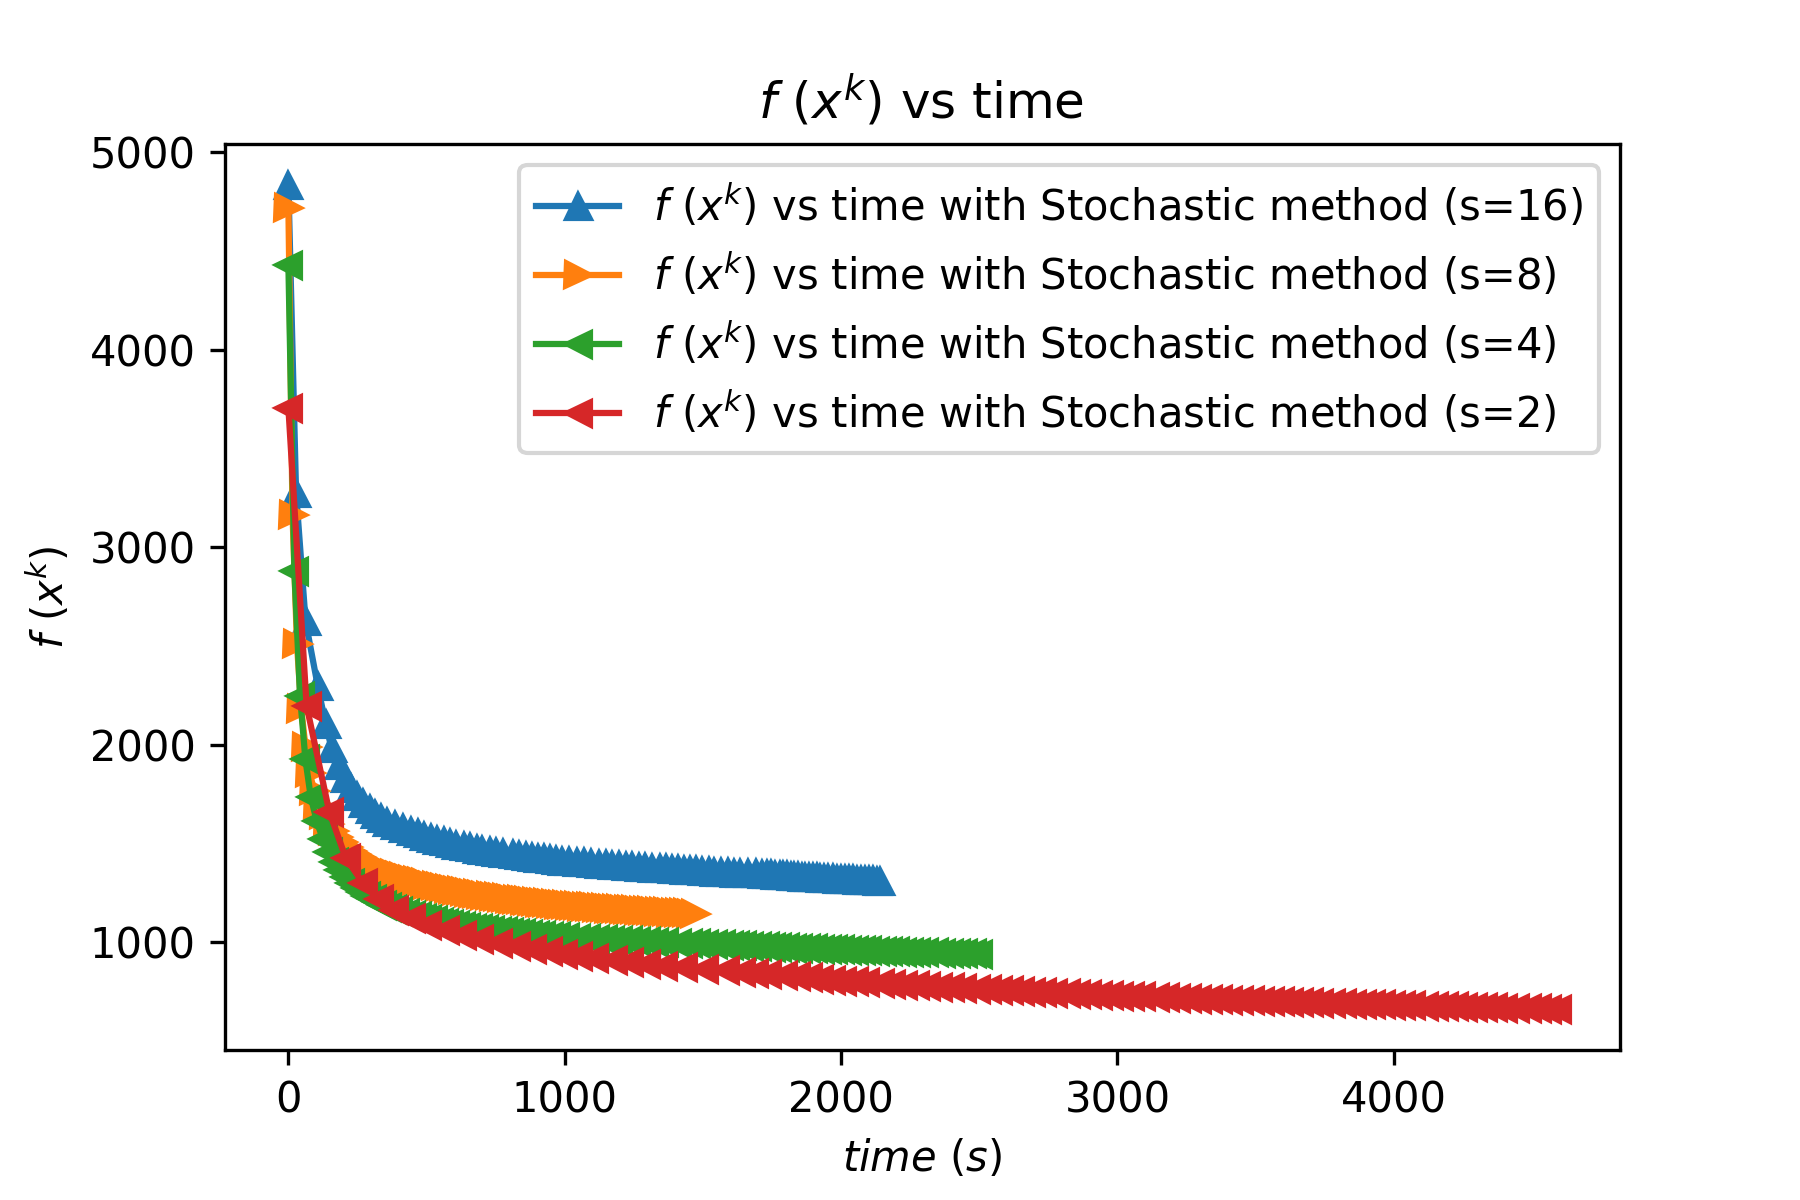
\includegraphics[width=3.5in]{pic18.png}
  \centering
  \caption{Comparision of $f(x^{k})$ vs. time for gradient descent accelerated by the Stochastic method with block size 2, 4, 8, 16.}
  \label{img18}
\end{figure}

\begin{figure}[h]
  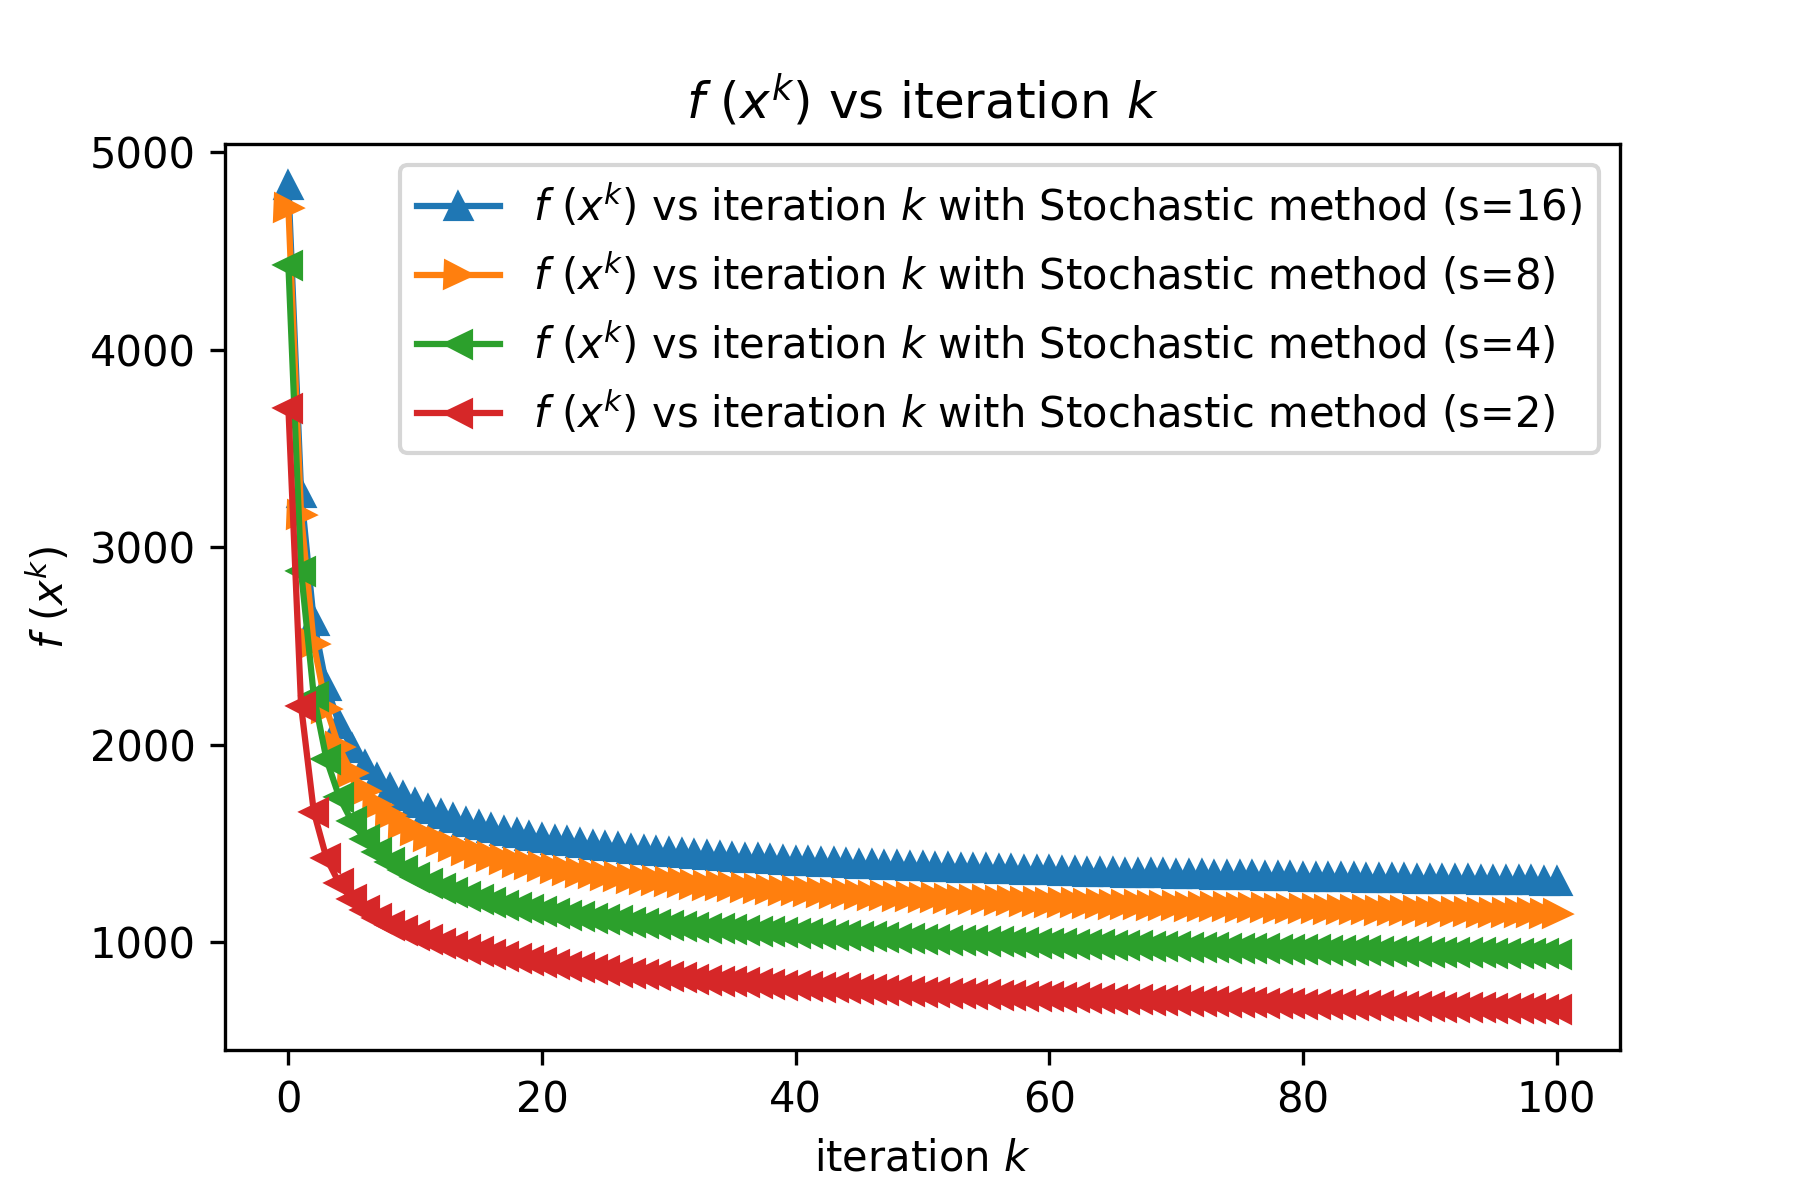
\includegraphics[width=3.5in]{pic19.png}
  \centering
  \caption{Comparision of $f(x^{k})$ vs. iteration k for gradient descent accelerated by the Stochastic method with block size 2, 4, 8, 16.}
  \label{img19}
\end{figure}

Considering the  $f(x^{k})$ vs. iteration k figure, it can be found that the speed of convergence increased as the size of block decreased. This is because the smaller the block size, the easier the best step size can reach its minimal value, and then the faster the image to fit its denoised state. However, looking at figure  \ref{img18}, it will be found that the overall time for 100 iterations is very different for those block sizes. 

According to figure \ref{img18}, the speed of convergence is fastest for block size 2, but the overall time for block sez 2 is the longest, which is almost the double of block size 4, or three times longer than the block size 8. The block size 4 will cause the shortest overall time, and enlarge or reduce the size of the block will both cause the overall time to be longer.

For all the previous experiments, the number of $\lambda$ is 0.9. This is because for gradient descent and gradient descent accelerated by the Nesterove method are both slow, which means for small $\lambda$ like 0.1, 0.2, 0.5, the noised image cannot converge as fast as the user wants. But for the stochastic method, the speed of convergence is fast, which causes the noised image being over-denoised, as shown in figure \ref{img20}.

\begin{figure}[h]
  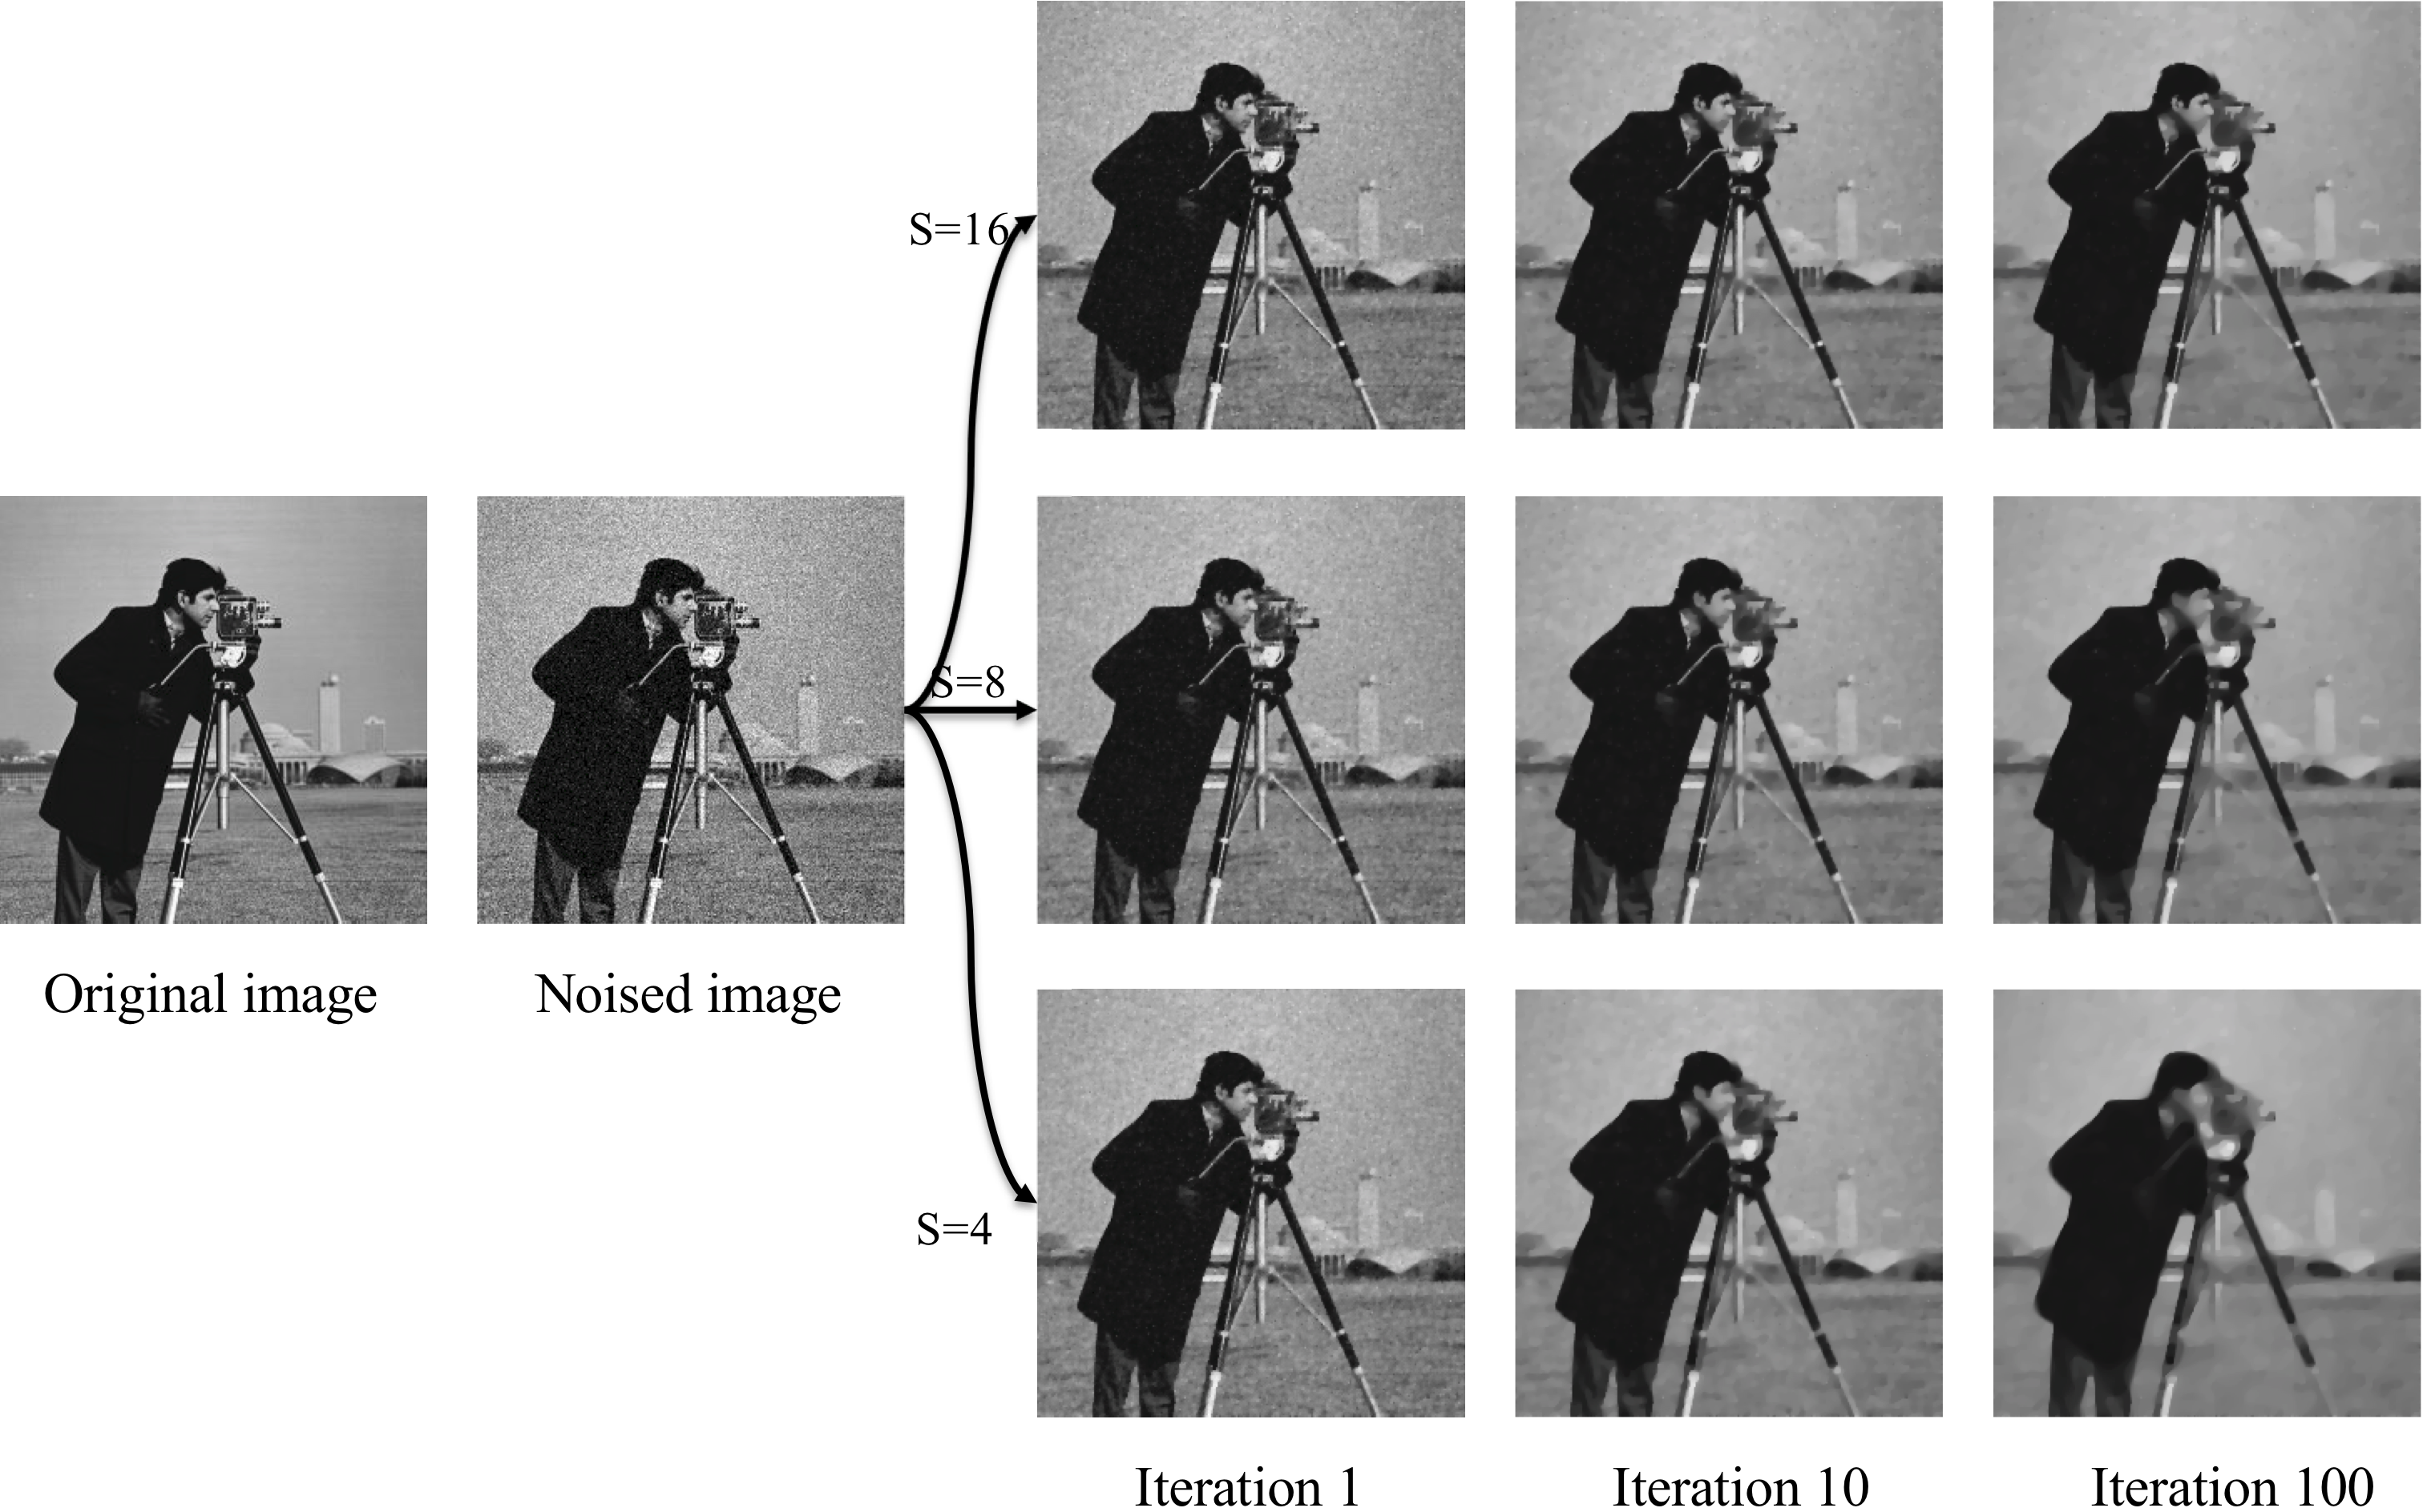
\includegraphics[width=5.5in]{pic20.png}
  \centering
  \caption{The original image, noised image, and three images are the denoised image with iteration 1, 10, and 100 with gradient descent accelerated by the Stochastic method with block size 4, 8, and 16.}
  \label{img20}
\end{figure}

As you can see, as the decrease of block size, the noised image being smother faster, but for block size 8 and 4, they are over-denoised. In this case, what we need to do is to decrease $\lambda$, and by experiment, $\lambda=0.1$ works well for block size 8 and 4.

\section{Large scale problem}

\subsection{The Weighted Stochastic method}
Stochastic method can significantly accelerate the denoising algorithm, which makes it possible to solve large-scale problems. But this method still takes more than 10 seconds to process a small 256x256 monochrome photo, which is unacceptable in practical applications. Therefore, we need a faster denoising method.

In practice, we found that for the stochastic method, the initial score of different windows is different, and the degree of difference of the points in the window can be judged by the initial score of the window. In order to make this theory simple and easy to understand, according to figure \ref{img21}, it can be found that for window sizes are 2x2, 4x4, 8x8, 16x16, 32x32, the place where is whiter is always the same place.

So we can sort the weights according to the color of the grid. A light-colored square means high weight. Those with high weight perform a few more operations when denois, and those with low weight do less operations. In order to achieve this goal, the random sampling method is selected, and the denois block is required to sample.
\begin{figure}[h]
  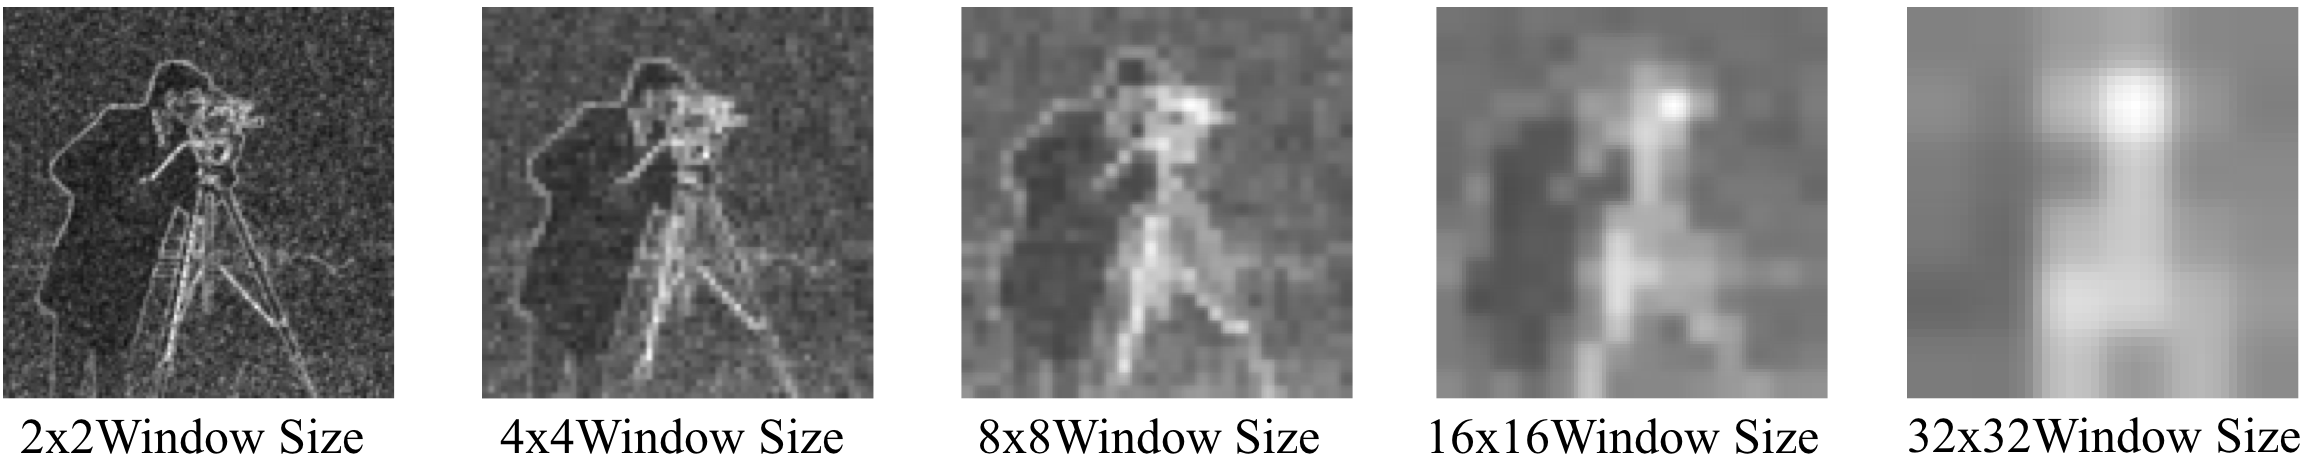
\includegraphics[width=5.5in]{pic21.png}
  \centering
  \caption{the scored figure of the “Camera Man” with different window size. (From left to right, the window sizes are 2x2, 4x4, 8x8, 16x16, 32x32).}
  \label{img21}
\end{figure}

\subsection{Random sampling for the Weighted Stochastic method}
The weight calculation method is shown below. First, the statistics are performed, and the statistical results are shown in the histogram (Figure \ref{img22}). By observing the figure \ref{img22}(a), (b), (c) and (d), you can find the score distribution of the square. It is an approximately normal distribution. The score is concentrated in the middle area, so the number of squares with a higher score is relatively small. The benefits of denoising these blocks with high scores will be greater than the benefits of denoising blocks with lower scores.
\begin{figure}[h]
  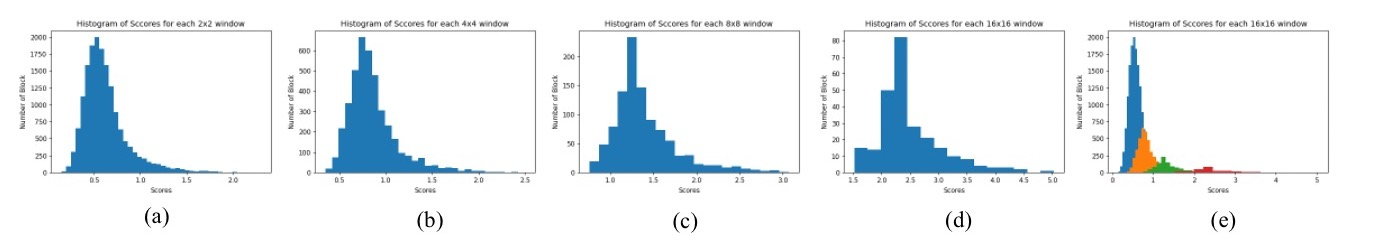
\includegraphics[width=5.5in]{pic22.jpg}
  \centering
  \caption{The score distribution of one figure with different window size (From (a) to (d), the window sizes are 2x2, 4x4, 8x8, 16x16, 32x32) and the plot on one single graph (e).}
  \label{img22}
\end{figure}
By observing the figure \ref{img22}(d), it can be found that the larger the window size, the higher the score. Therefore, a function is needed to correct the histogram so that the score is not too high for the high score and not too low for the low score. Finally, perform denoising calculation after sampling according to weight. Or the total number of running squares is the total number of image squares set as 1 iteration.

The random sampling algorithm based on the score is as follows.
\begin{python}
def getProbArray(x, f, fun, lambda_, side):
    weight = getWeightTable(x, f, fun, lambda_, side)
    max_w = weight.max()
    min_w = weight.min()
    hist_data = np.array(weight)
    hist_data=(hist_data+hist_data.mean())
    hist_data=hist_data/hist_data.sum()
    prob_list = []
    pos_list = []
    for i in range(hist_data.shape[0]):
        for j in range(hist_data.shape[1]):
            pos_list.append([i,j])
            prob_list.append(hist_data[i,j])
    return pos_list, prob_list
  
  def randomChoise(pos_list, prob_list):
    p = np.array(prob_list)
    index = np.random.choice(list(range(len(prob_list))), p = p.ravel())
    return pos_list[index]
\end{python}

\subsection{Parallel Computing}
For large-scale problems, parallel computing is a good way to increase speed. For large images, we first need to split the color of the image. As shown in figure \ref{img23}, layer the color image according to the red, green and blue layers to get three monochrome images. But these monochrome pictures are still very large, so parallel computing is needed to increase the speed.
\begin{figure}[h]
  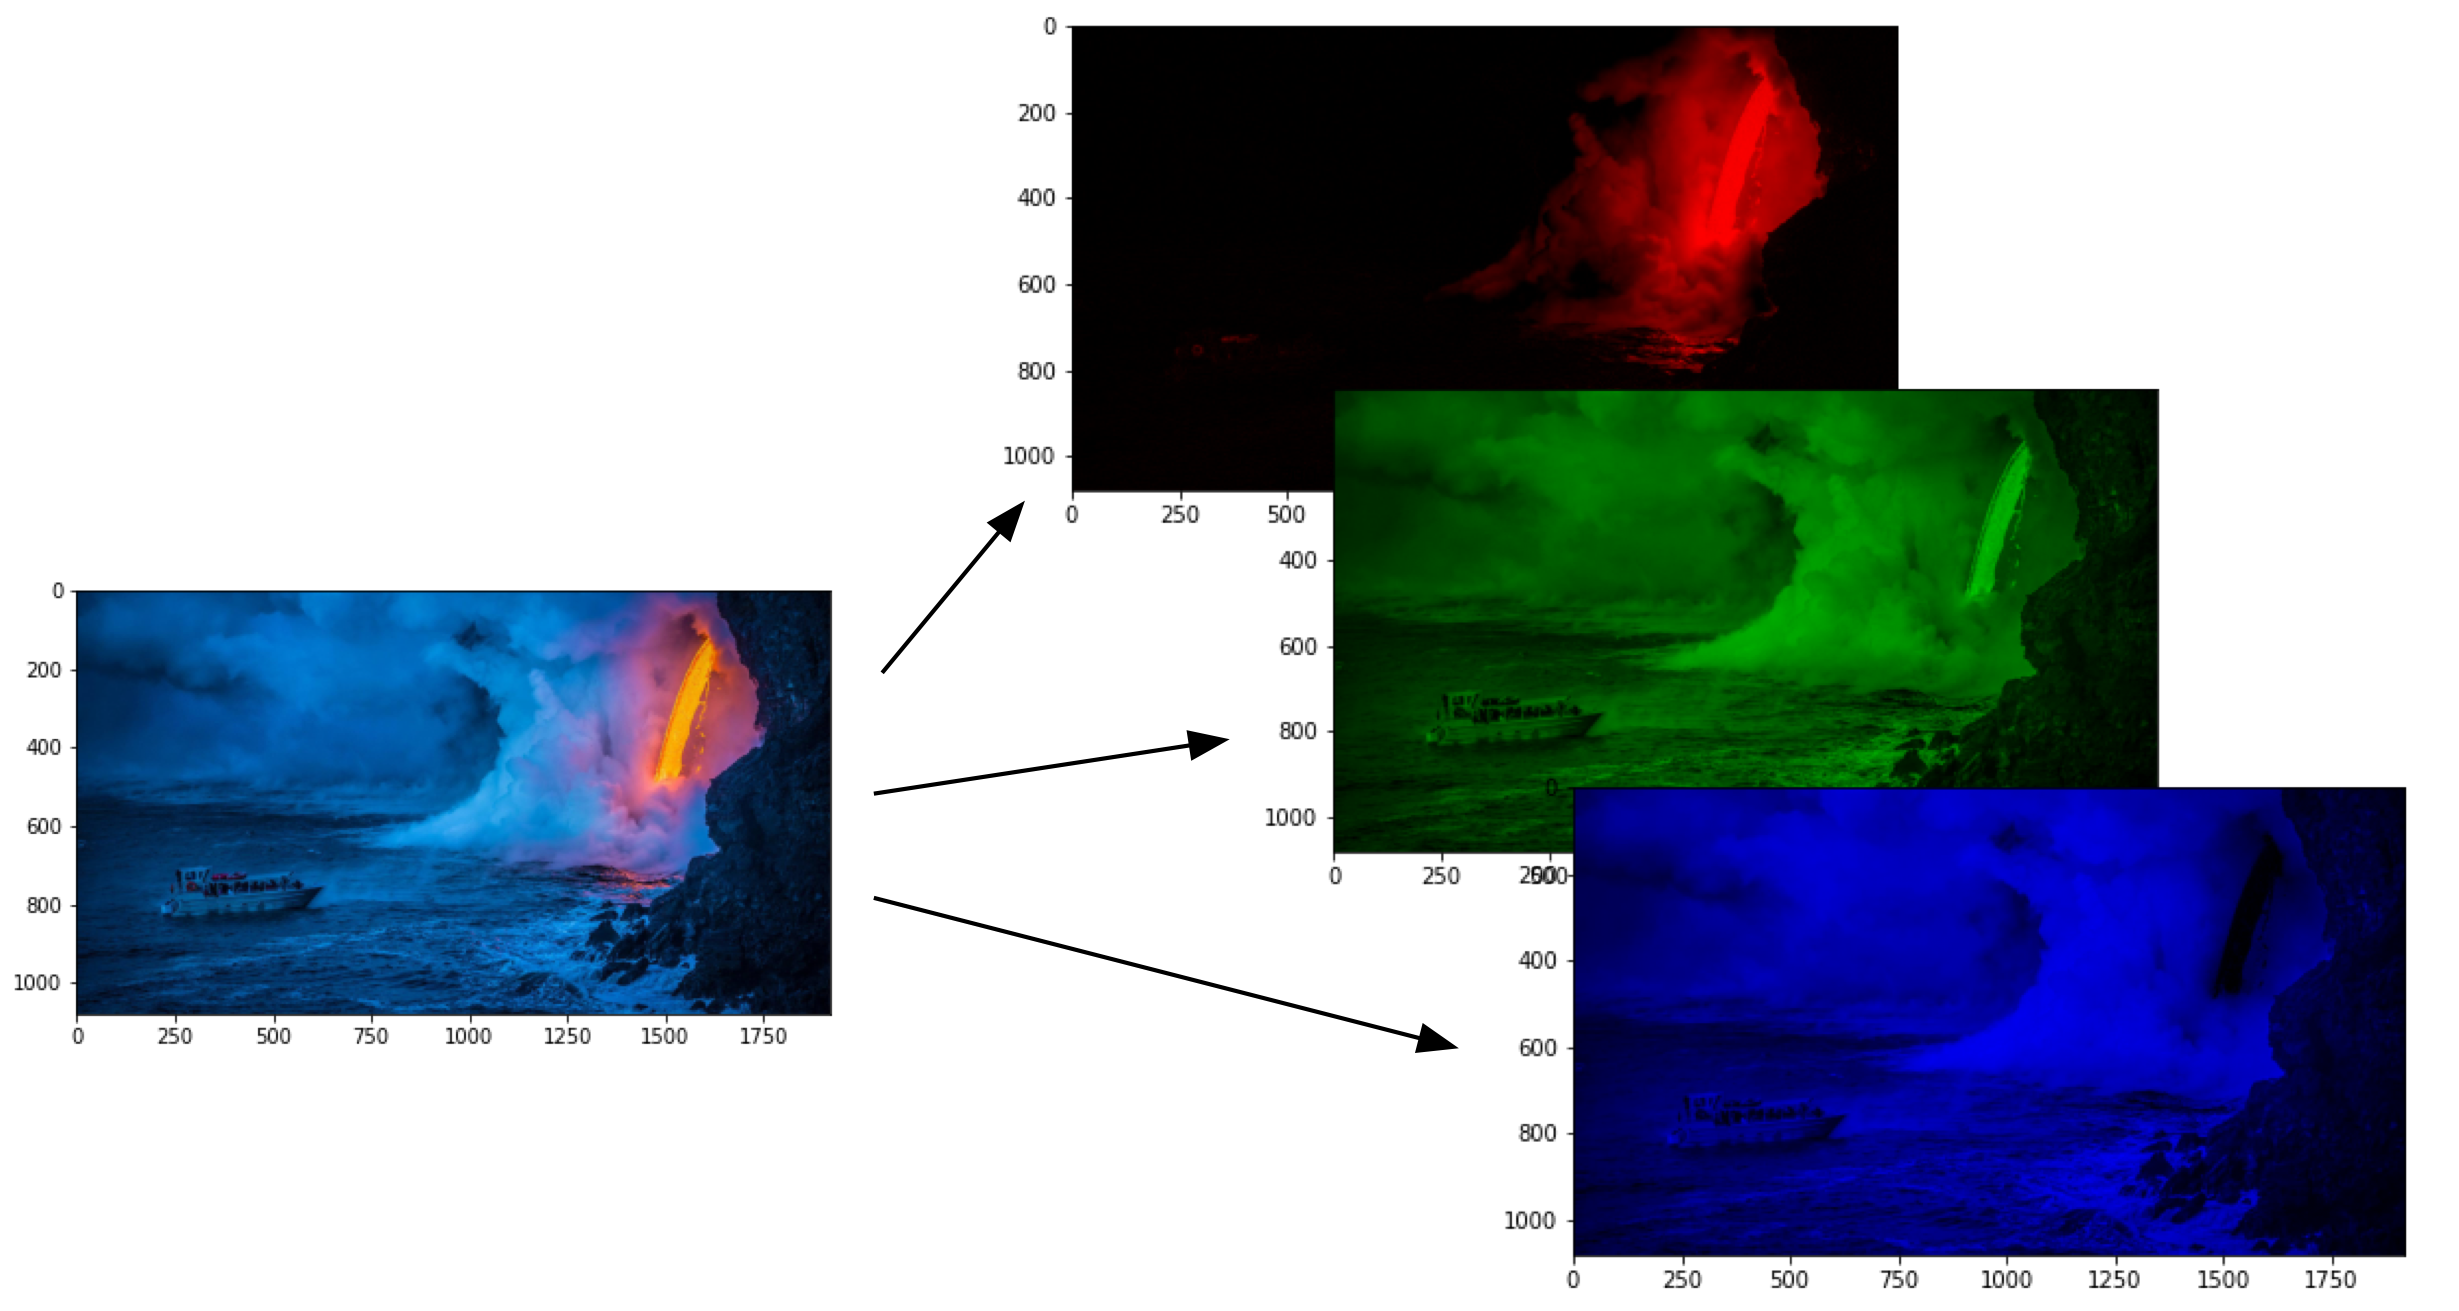
\includegraphics[width=3.5in]{pic23.png}
  \centering
  \caption{Layer the color pictures according to the RGB layers to get three monochrome pictures.}
  \label{img23}
\end{figure}
For large-scale problems, distributed computing is required. Parallel computing can be simply defined as using multiple computing resources to solve a computing problem at the same time. Because we use the stochastic method, the denoising problem can be broken down into discrete and concurrently solvable parts. By cutting the big picture into multiple windows of equal size, and then grouping these windows into different computer cores for calculation. The result is that each part of the instructions are executed simultaneously on different CPUs.

My computer is MacBook Pro 2015 (2 Cores, 2.7 GHz). Because there is only 2 cores, we can only use 2 process to do parallel computing.

Therefore, my python program divides the windows generated by the picture into two groups, and hands them to the two system cores for python parallel calculation. After the picture is divided into blocks, the windows are grouped according to high and low strength, and try to divide them into two groups with the same total score as much as possible. Then the two groups are calculated separately on different calculations and cores, and each round of calculation is completed and merged. For multiple computers or computers with multiple cores, you can get faster speeds. Figure \ref{img24} shows the acceleration method when multiple cores are used.

\begin{figure}[h]
  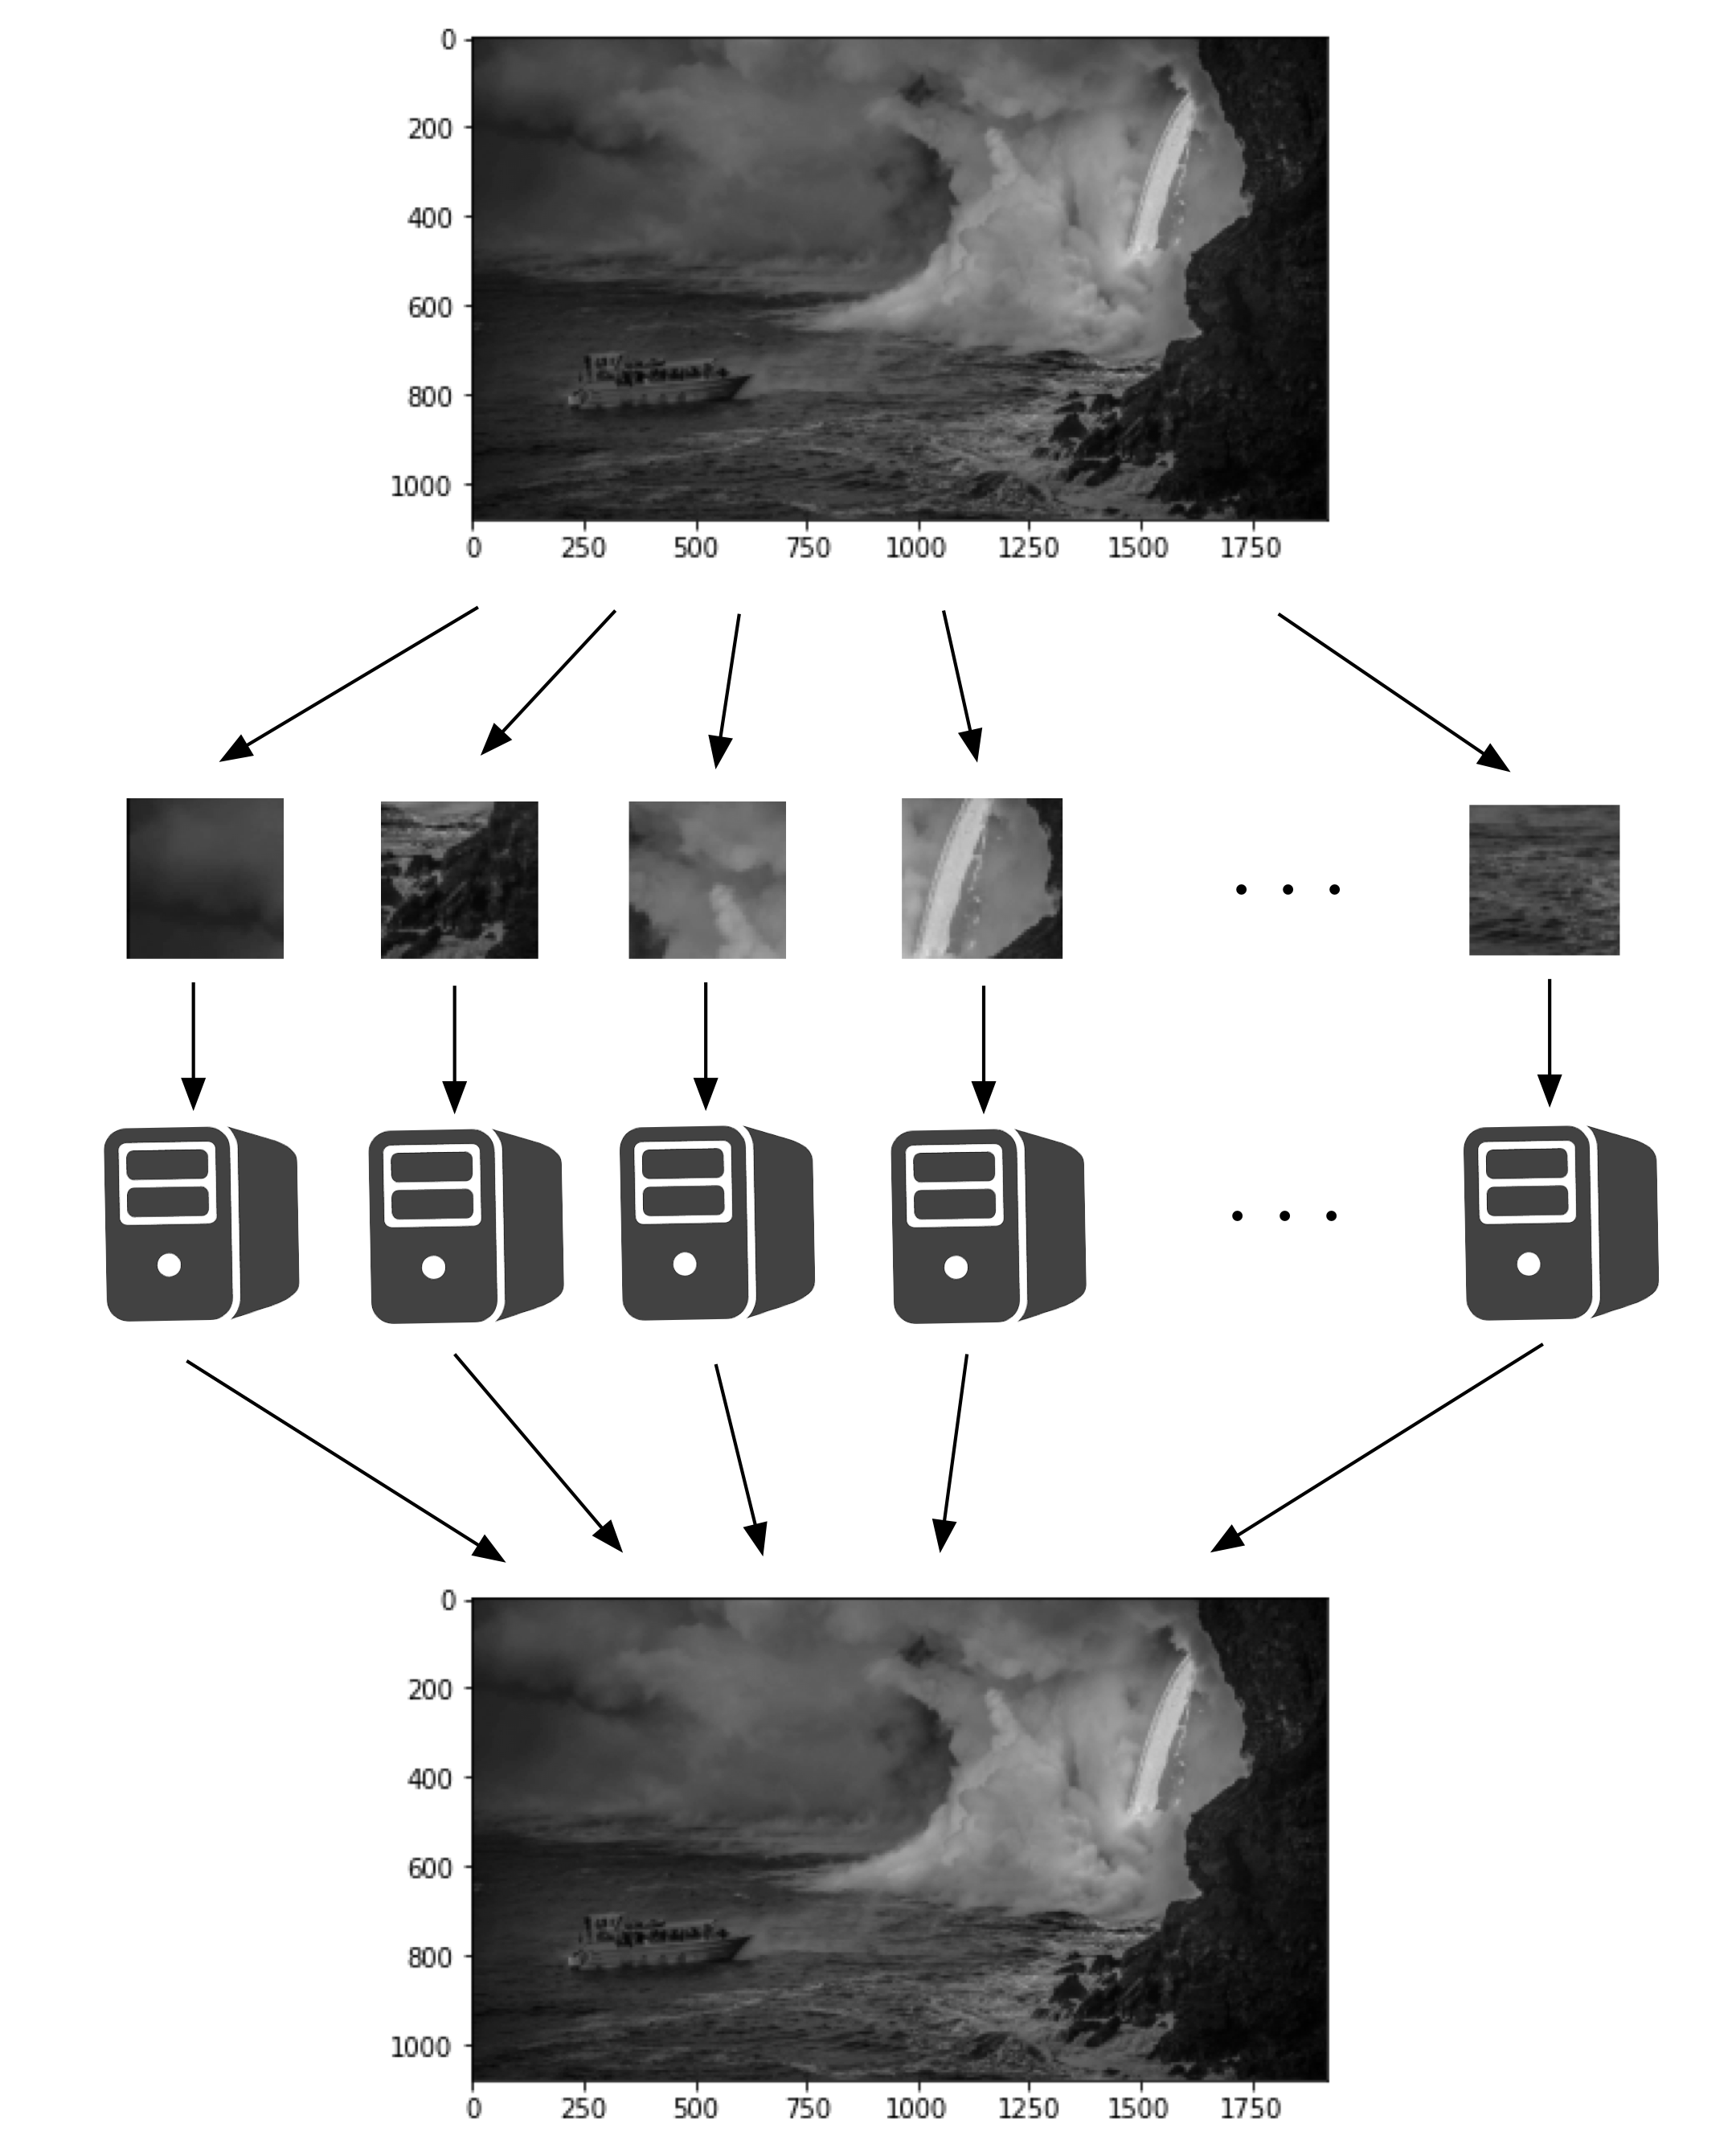
\includegraphics[width=3.5in]{pic24.png}
  \centering
  \caption{Schematic diagram of parallel calculation of denoising algorithm accelerated by weighted stochastic method.}
  \label{img24}
\end{figure}

\subsection{Comparison of gradient descent and gradient descent accelerated by Parallel Computing method}
First, the $f(x^{k})$ vs. time and  $f(x^{k})$ vs. iteration k are presented to show the speed of convergence, in figure \ref{img25} and figure \ref{img26}, compared with the general gradient descent, gradient descent accelerated by the Nesterov method, gradient descent accelerated by the Stochastic method. Figure \ref{img25} shows that the total time of parallel calculation will be faster than single-core calculation, but comparing figure \ref{img26}, it can be found that there is no significant improvement in $f(x^{k})$ vs. iteration k. This is normal, because parallel computing does not reduce the amount of calculation required, but only reduces the required calculation time. However, it is found in figure \ref{img25} that the time reduction of parallel computing is not as normal, only about a quarter of the original. This is because a single host is performing parallel computing while also having other computing tasks. So the final conclusion is that parallel computing can indeed reduce the total calculation time required.
\begin{figure}[h]
  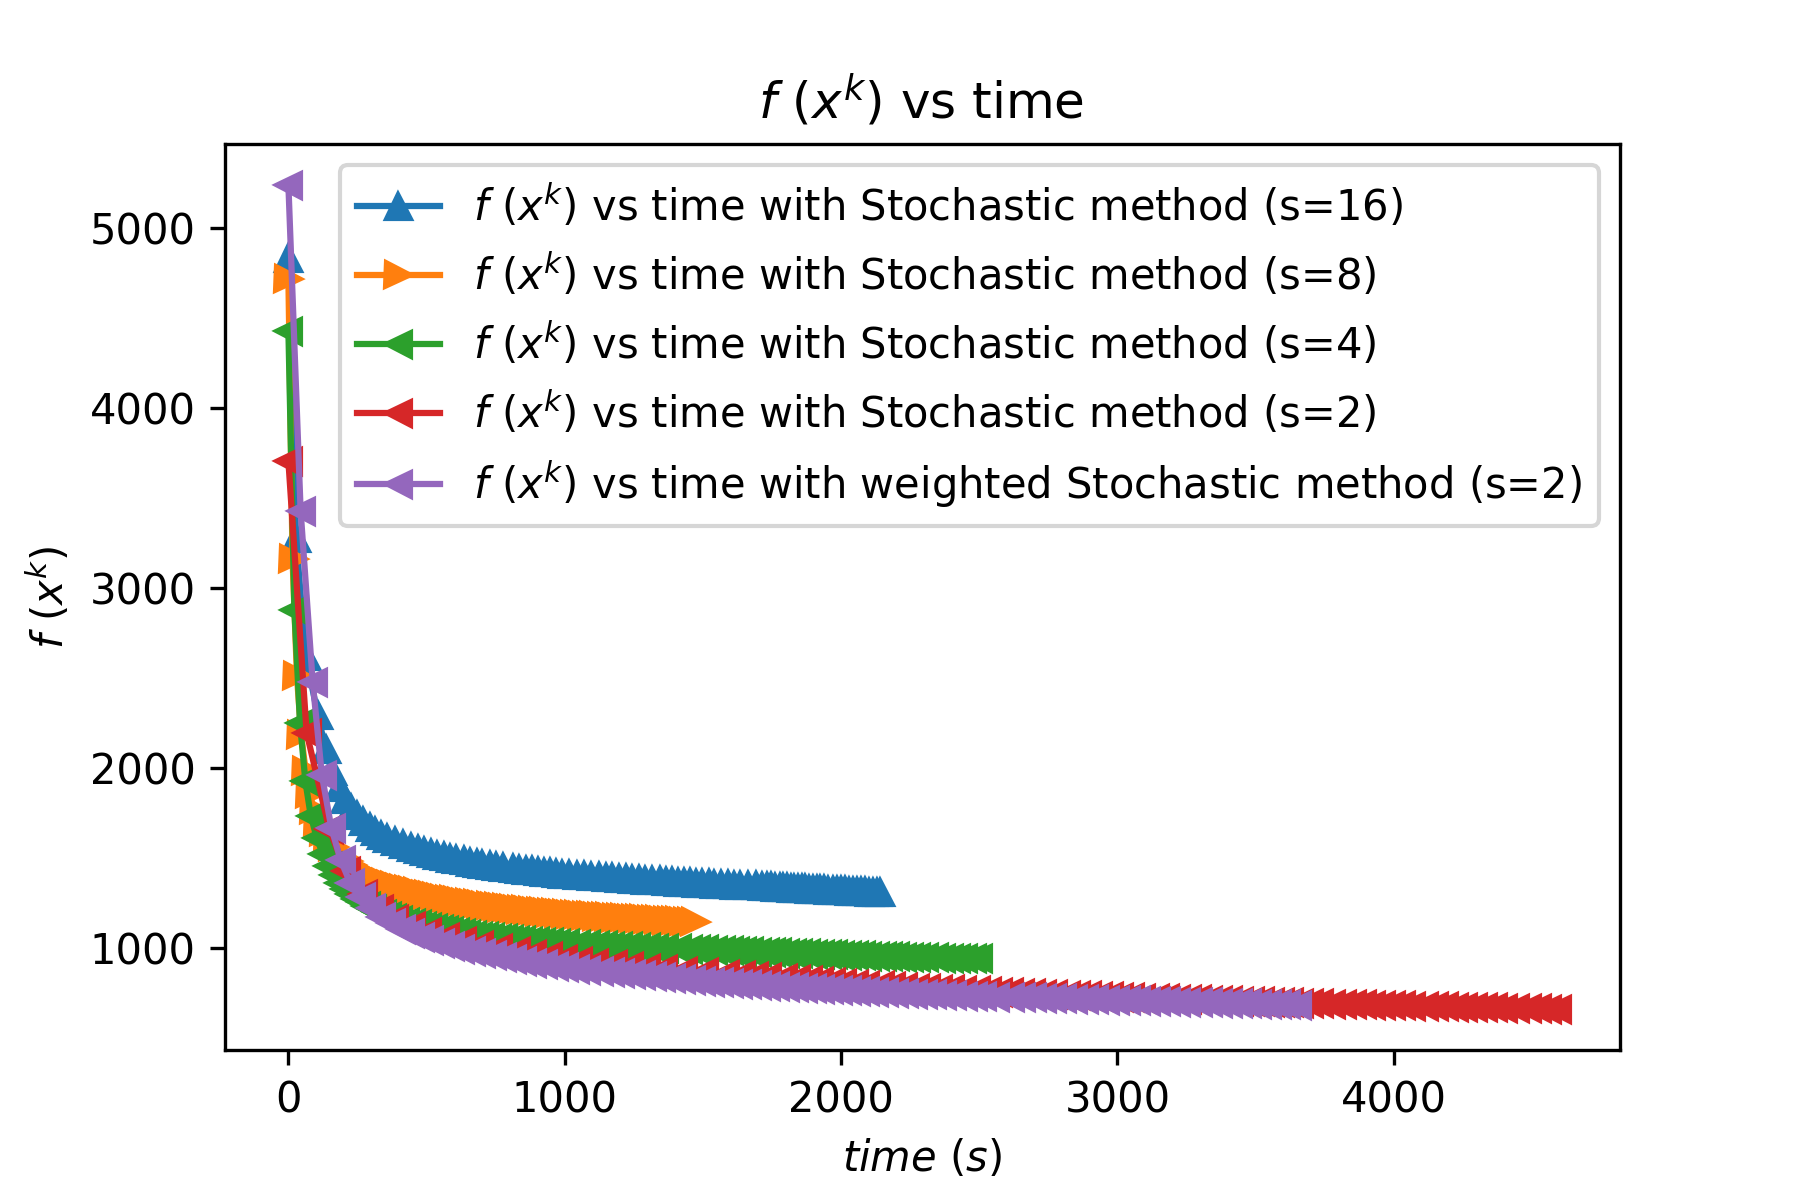
\includegraphics[width=3.5in]{pic25.png}
  \centering
  \caption{Comparison of $f(x^{k})$ vs. time for gradient descent, gradient descent accelerated by the Nesterov method, gradient descent accelerated by the Stochastic method, and gradient descent accelerated by the weighted Stochastic method.}
  \label{img25}
\end{figure}
\begin{figure}[h]
  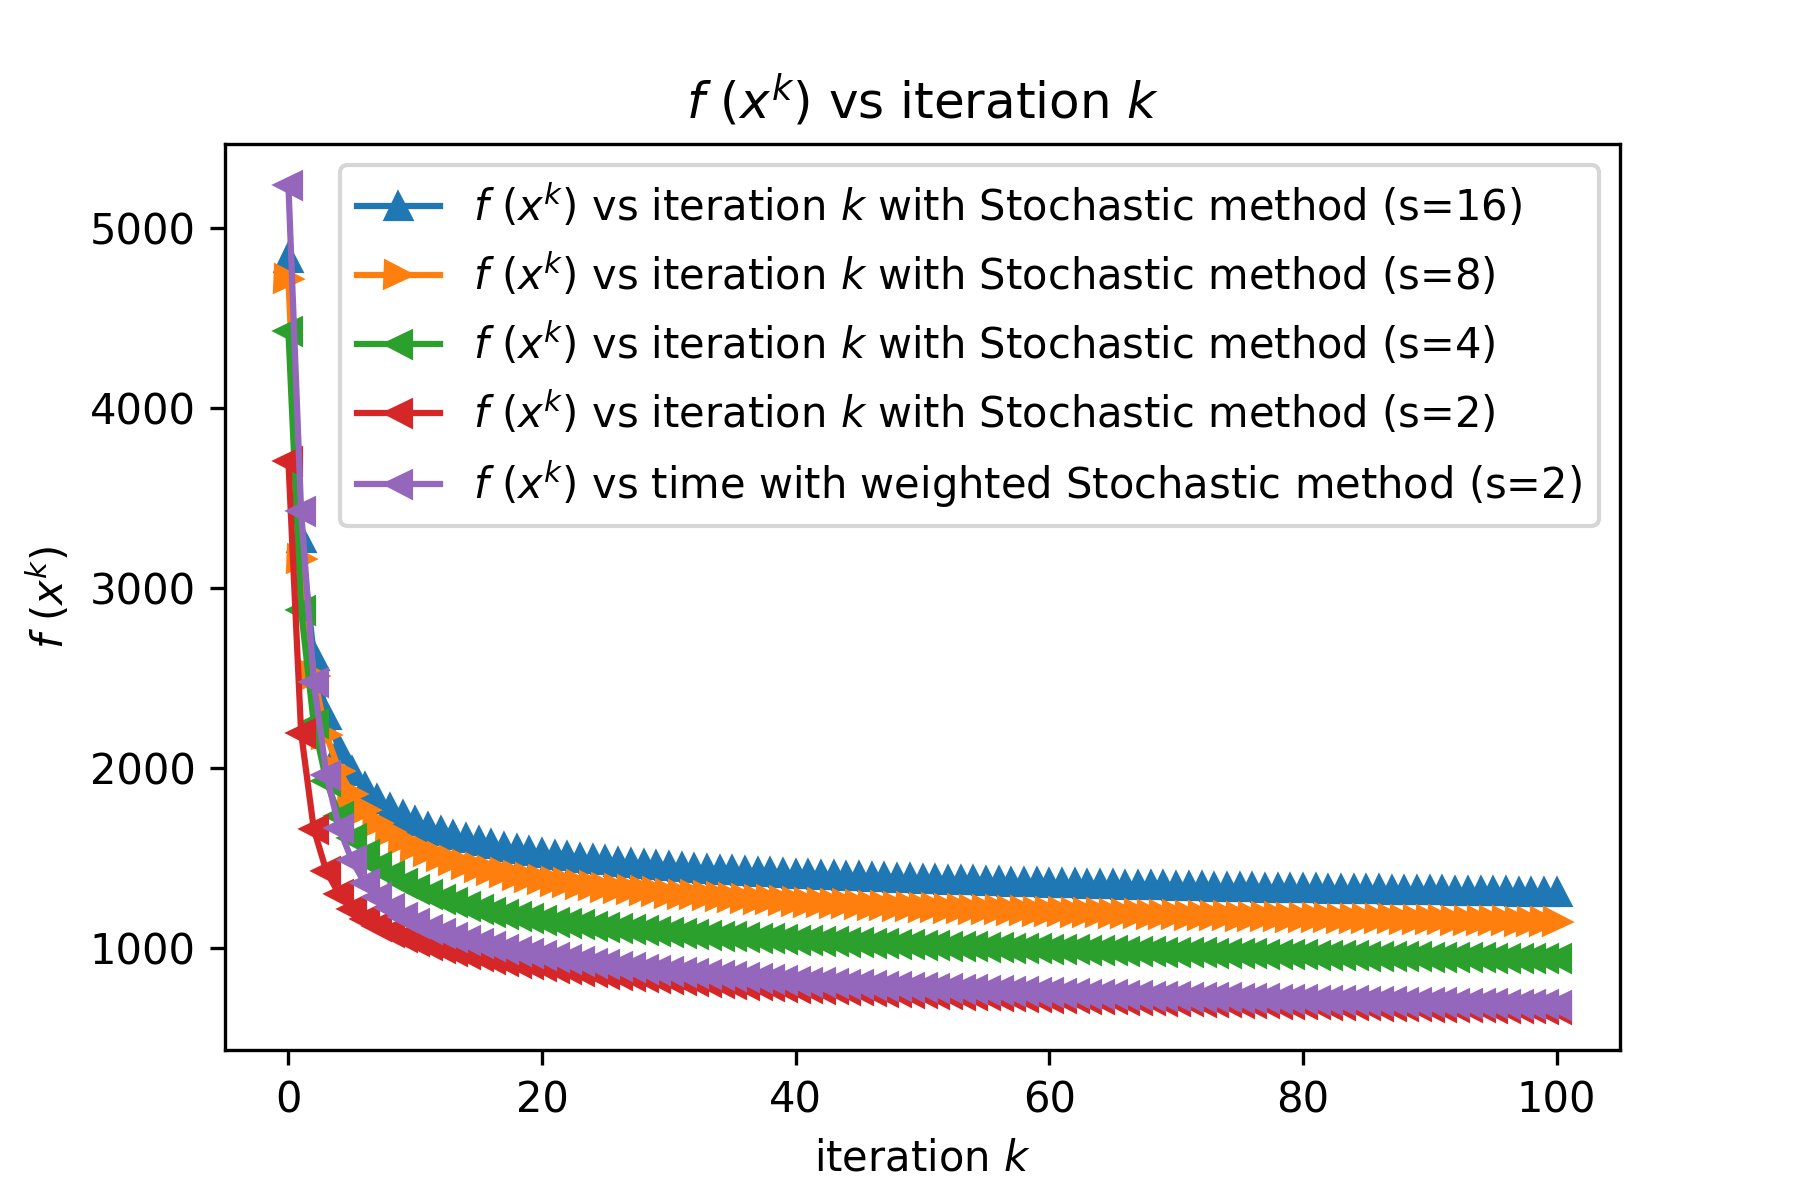
\includegraphics[width=3.5in]{pic26.png}
  \centering
  \caption{Comparison of $f(x^{k})$ vs. time for gradient descent, gradient descent accelerated by the Nesterov method, gradient descent accelerated by the Stochastic method, and gradient descent accelerated by the weighted Stochastic method.}
  \label{img26}
\end{figure}
\section{Conclusion}
In this project, a variety of algorithms are applied to the field of image denoising. From the simplest gradient descent to various gradient descent acceleration algorithms, such as Nesterov and stochastic acceleration algorithms. Finally, parallel computing was tried to speed up the computing speed. Through these algorithms, the importance of optimization algorithms is understood. This project helped me understand the optimization algorithm and its practical application more deeply.

The code of this project is based on python3.6 and can run on higher versions of python. The operating environment is MacOS, and after testing, the same effect can be achieved on Linux. However, some parallel computing part of the code cannot run on windows. All codes are developed on the Jupyter Lab platform, which can be visually edited in real-time and save time.

Finally, I would like to appreciate Professor Huang for teaching the wonderful class and answering my questions, and thanks all TAs for their help!


\bibliographystyle{plainnat}
\bibliography{VE485_project}
\end{document}
